\documentclass[11pt,a4paper]{article}
\usepackage{graphicx}
\DeclareGraphicsExtensions{.pdf, .png, .jpg}
\usepackage{style}

\renewcommand{\thesection}{S\arabic{section}}
\renewcommand{\thefigure}{S\arabic{figure}}
\renewcommand{\thetable}{S\arabic{table}}

\sloppy

\title{The Influence of Temperature on Ozone Production under varying \ce{NO_x} Conditions -- a modelling study: Supplementary Material}
\author[1]{J. Coates}
\author[1]{K. A. Mar}
\author[2]{N. Ojha}
\author[1]{T. M. Butler}
\affil[1]{Institute for Advanced Sustainability Studies, Potsdam, Germany}
\affil[2]{Atmospheric Chemistry Department, Max Planck Institute for Chemistry, Mainz, Germany}

\renewcommand\Authands{ and }

\begin{document}

\maketitle

\section{Allocation of Benelux AVOC emissions to Mechanism Species}
Anthropogenic NMVOC emissions over Benelux specified by the TNO\_MACCIII emission inventory \citep{Kuenen:2014} were translated to MCM~v3.2 emissions (Table~\ref{t:Benelux_MCM_emissions}).
The MCM~v3.2 emissions for each initial species were translated to emissions of mechanism species into CRI~v2, MOZART-4 and RADM2 chemical mechanisms by weighting with the carbon numbers (Tables~\ref{t:CRI_NMVOC_emissions} -- \ref{t:RADM2_NMVOC_emissions}).
The allocation of MCM~v3.2 emissions into CB05 species followed the recommendations of \citet{Yarwood:2005} (Table~\ref{t:CB05_NMVOC_emissions}).
{
    \begin{landscape}%
        \centering%
        \tiny
\begin{longtable}{lllllllllllllll}
    \caption{Speciated TNO\_MACCIII emissions for Benelux AVOC and BVOC emissions (molecules~cm$^{-2}$~s$^{-1}$) mapped to MCM~v3.2 species \citep{Kuenen:2014}.}\\%
	\hline \hline
	\textbf{Type} & \textbf{MCM.Species} & \textbf{SNAP.1} & \textbf{SNAP.2} & \textbf{SNAP.34} & \textbf{SNAP.5} & \textbf{SNAP.6} & \textbf{SNAP.71} & \textbf{SNAP.72} & \textbf{SNAP.73} & \textbf{SNAP.74} & \textbf{SNAP.8} & \textbf{SNAP.9} & \textbf{BVOC} & \textbf{Total}\\
	\endhead
	\hline
	Ethane & C2H6 & 9.85e+08 & 1668300000 & 9.18e+09 &  &  & 9.67e+08 & 2.96e+08 & 63860000 &  & 3.45e+08 & 210200000 &  & 1.3728e+10 \\
	\hline Propane & C3H8 & 2.886e+09 & 1086600000 & 2.573e+09 & 1.041e+11 & 9.72e+08 & 47090000 & 202400000 & 638600000 & 62710000 & 249700000 & 75200000 &  & 1.129e+11 \\ \hline
	\multirow{2}{*}{Butanes} & NC4H10 & 2.127e+09 & 882870000 & 949270000 & 6.11e+11 & 3.61e+09 & 1.048e+09 & 209500000 &  & 1037800000 & 315300000 & 42200000 &  & 6.21e+11 \\
	 & IC4H10 & 258600000 & 309660000 & 232311000 & 1.486e+11 & 163700000 & 489100000 & 97500000 &  & 483900000 & 157900000 & 42200000 &  & 1.509e+11 \\
	\hline \multirow{3}{*}{Pentanes} & NC5H12 & 1.783e+09 & 1014960000 &  & 4.548e+11 &  & 6.27e+08 & 8.4e+07 &  & 521500000 & 118200000 & 14890000 &  & 4.589e+11 \\
	 & IC5H12 & 7.52e+08 & 544340000 &  & 2.718e+11 &  & 1.216e+09 & 163500000 &  & 1011700000 & 225600000 & 14890000 &  & 2.762e+11 \\
	 & NEOP &  &  &  &  &  &  &  &  &  &  & 14890000 &  & 14890000 \\
	\hline \parbox[t]{2mm}{\multirow{14}{*}{\rotatebox[origin=c]{90}{Hexane and Higher Alkanes}}} & NC6H14 & 954100000 & 57390000 & 1.211e+09 & 6.49e+10 & 3.162e+09 & 2.207e+09 & 1.246e+09 &  & 193450000 & 4.26e+08 & 5160000 &  & 7.44e+10 \\
	 & M2PE &  &  & 156600000 & 9.98e+09 & 6.66e+08 &  &  &  &  & 7.08e+08 & 2215000 &  & 1.151e+10 \\
	 & M3PE &  &  & 117100000 & 4.989e+09 & 6.66e+08 &  &  &  &  & 4.26e+08 &  &  & 6.2e+09 \\
	 & NC7H16 & 409520000 & 98740000 & 5.71e+08 & 6.97e+10 & 1.146e+09 & 363500000 & 205300000 &  & 31790000 & 121900000 & 26040000 &  & 7.28e+10 \\
	 & M2HEX &  &  &  &  & 4.3e+08 & 2.83e+08 & 159500000 &  & 24710000 & 182900000 &  &  & 1.08e+09 \\
	 & M3HEX &  &  &  &  & 4.3e+08 & 2.02e+08 & 1.14e+08 &  & 17634000 & 121900000 &  &  & 8.86e+08 \\
	 & M22C4 &  &  &  &  &  &  &  &  &  & 141800000 &  &  & 141800000 \\
	 & M23C4 &  &  &  &  &  &  &  &  &  & 141800000 &  &  & 141800000 \\
	 & NC8H18 &  &  & 235300000 & 5.18e+10 & 125600000 & 319500000 & 179700000 &  & 27890000 & 6.95e+08 & 8900000 &  & 5.33e+10 \\
	 & NC9H20 &  &  & 131200000 &  & 3.02e+09 &  &  &  &  &  & 2969000 &  & 3.148e+09 \\
	 & NC10H22 &  &  & 1.66e+08 &  & 5.85e+09 & 142200000 & 80300000 &  & 12458000 &  & 4460000 &  & 6.25e+09 \\
	 & NC11H24 &  &  & 64600000 &  & 2.387e+09 & 51830000 & 29280000 &  & 4536000 & 78100000 & 1625000 &  & 2.617e+09 \\
	 & NC12H26 &  &  &  &  & 168500000 & 8.45e+08 & 476900000 &  & 74100000 & 71700000 &  &  & 1.637e+09 \\
	 & CHEX &  & 91490000 & 4e+07 &  & 6.82e+08 &  &  &  &  &  & 1506000 &  & 8.15e+08 \\
	\hline Ethene & C2H4 & 212300000 & 3695700000 & 3.368e+10 &  &  & 5.341e+09 & 3.807e+09 & 342500000 &  & 4.62e+09 & 1.9e+08 &  & 5.188e+10 \\ \hline
	Propene & C3H6 & 141700000 & 868200000 & 6.59e+08 &  &  & 1.876e+09 & 634800000 & 151810000 &  & 7.86e+08 & 54500000 &  & 5.18e+09 \\
	\hline \parbox[t]{2mm}{\multirow{11}{*}{\rotatebox[origin=c]{90}{Higher Alkenes}}} & HEX1ENE & 21050000 & 15773000 &  &  &  &  &  &  &  &  & 21810000 &  & 58703000 \\
	 & BUT1ENE &  & 22154000 & 240400000 &  &  &  &  &  &  & 24510000 &  &  & 286604000 \\
	 & MEPROPENE &  &  &  &  &  &  &  &  &  & 12260000 &  &  & 12260000 \\
	 & TBUT2ENE &  &  &  &  &  &  &  &  &  & 12260000 &  &  & 12260000 \\
	 & CBUT2ENE &  &  &  &  &  &  &  &  &  & 12260000 &  &  & 12260000 \\
	 & CPENT2ENE &  & 6961000 &  &  &  &  &  &  &  & 4902000 &  &  & 11861000 \\
	 & TPENT2ENE &  & 6961000 &  &  &  &  &  &  &  & 4902000 &  &  & 11861000 \\
	 & PENT1ENE &  & 6328000 & 6186000 &  &  &  &  &  &  & 19630000 &  &  & 32171000 \\
	 & ME2BUT2ENE &  & 3793000 &  &  &  &  &  &  &  & 9800000 &  &  & 13581000 \\
	 & ME3BUT1ENE &  & 3793000 &  &  &  &  &  &  &  & 9800000 &  &  & 13581000 \\
	 & ME2BUT1ENE &  & 2525500 &  &  &  &  &  &  &  &  &  &  & 2525500 \\
	\hline Ethyne & C2H2 & 2697000 & 1252200000 & 426600000 &  &  & 4.975e+09 & 1.795e+09 & 134690000 & 252500000 & 1.614e+09 & 71500000 &  & 1.051e+10 \\ \hline
	Benzene & BENZENE & 269600000 & 1.006e+09 & 8.3e+08 & 1.621e+10 &  & 1.197e+09 & 228300000 &  & 35380000 & 2.83e+08 & 36540000 &  & 2.014e+10 \\
	\hline Toluene & TOLUENE & 252700000 & 372760000 & 84400000 & 1.375e+10 & 6.8e+09 & 2.708e+09 & 1.45e+08 &  & 30030000 & 193900000 & 24100000 &  & 2.435e+10 \\ \hline
	\multirow{3}{*}{Xylenes} & MXYL & 1.05e+08 & 21179000 & 1669300 & 1.994e+09 & 3.93e+09 & 5.77e+08 & 61040000 &  & 4735000 & 70200000 & 4880000 &  & 6.78e+09 \\
	 & OXYL & 23330000 & 21179000 & 669700 & 1.994e+09 & 9.84e+08 & 5.77e+08 & 61040000 &  & 4735000 & 57100000 & 2924000 &  & 3.717e+09 \\
	 & PXYL &  & 21179000 & 669700 & 1.994e+09 & 9.84e+08 & 432900000 & 45800000 &  & 3551000 & 70200000 & 3909000 &  & 3.556e+09 \\
	\hline \multirow{3}{*}{Trimethylbenzenes} & TM123B & 18550 & 1304500 &  &  & 6.6e+07 & 99200000 &  &  &  & 3330000 & 441000 &  & 170200000 \\
	 & TM124B & 18550 & 1304500 & 56100000 &  & 224600000 & 4.16e+08 &  &  &  & 7760000 & 589000 &  & 7.06e+08 \\
	 & TM135B & 18550 & 1304500 &  &  & 6.6e+07 & 158600000 &  &  &  & 3330000 & 589000 &  & 229900000 \\
	\hline \parbox[t]{2mm}{\multirow{11}{*}{\rotatebox[origin=c]{90}{Other Aromatics}}} & EBENZ & 35100000 &  & 63400000 &  & 179400000 & 430600000 & 341600000 & 119530 &  & 8e+08 & 5250000 &  & 1.856e+09 \\
	 & PBENZ &  &  &  &  & 39600000 & 380600000 & 301500000 & 105570 &  & 128500000 & 2311000 &  & 8.53e+08 \\
	 & IPBENZ &  &  &  &  & 145300000 &  &  &  &  & 128500000 & 2311000 &  & 276300000 \\
	 & PETHTOL &  &  &  &  & 13210000 &  &  &  &  & 257500000 &  &  & 270300000 \\
	 & METHTOL &  &  &  &  & 39600000 &  &  &  &  & 257500000 &  &  & 296300000 \\
	 & OETHTOL &  &  &  &  &  &  &  &  &  & 192800000 &  &  & 192800000 \\
	 & DIET35TOL &  &  &  &  &  & 8.05e+08 & 637600000 & 223800 &  &  &  &  & 1.443e+09 \\
	 & DIME35EB &  &  &  &  & 224700000 & 99300000 & 78700000 & 27540 &  &  &  &  & 4.03e+08 \\
	 & STYRENE &  &  & 64600000 &  & 45700000 & 91500000 & 72500000 & 25440 &  &  &  &  & 275100000 \\
	 & BENZAL &  &  &  &  &  & 153900000 & 121900000 & 42690 &  &  &  &  & 275900000 \\
	 & PHENOL &  &  & 71500000 &  &  &  &  &  &  &  &  &  & 71500000 \\
	\hline Formaldehyde & HCHO & 611400000 & 2195300000 &  &  &  & 1.177e+09 & 1.781e+09 & 85260000 &  & 2.9e+09 & 29490000 &  & 8.77e+09 \\ \hline
	\parbox[t]{2mm}{\multirow{9}{*}{\rotatebox[origin=c]{90}{Other Aldehydes}}} & CH3CHO & 11780000 & 130090000 & 73750000 &  &  & 318400000 & 7.39e+08 & 16383000 &  & 6.8e+08 & 6860000 &  & 1.976e+09 \\
	 & C2H5CHO & 6710000 & 98630000 &  &  &  & 53670000 & 124600000 & 2752000 &  & 257700000 & 5200000 &  & 5.49e+08 \\
	 & C3H7CHO & 38630 & 79420000 &  &  &  &  &  &  &  & 207600000 & 4190000 &  & 292100000 \\
	 & IPRCHO & 38630 & 79420000 &  &  &  &  &  &  &  & 138400000 & 4190000 &  & 222100000 \\
	 & C4H9CHO & 32340 & 66550000 &  &  &  &  &  &  &  &  & 3504000 &  & 70050000 \\
	 & ACR & 49770 & 102260000 &  &  &  & 83300000 & 193800000 & 4282000 &  &  & 5390000 &  & 388800000 \\
	 & MACR & 39730 & 81710000 &  &  &  &  &  &  &  &  & 4310000 &  & 86110000 \\
	 & C4ALDB & 39730 & 81710000 &  &  &  & 44510000 & 103300000 & 2287000 &  &  & 4310000 &  & 236100000 \\
	 & MGLYOX &  &  &  &  &  &  &  &  &  & 138500000 &  &  & 138500000 \\
	\hline Alkadienes and & C4H6 & 67600000 & 771300000 & 4.74e+09 & 2.221e+11 &  & 2.505e+09 & 7.78e+08 & 245800000 & 458800000 & 1.033e+09 & 52800000 &  & 2.332e+11 \\
	Other Alkynes & C5H8 &  &  &  &  &  &  &  &  &  &  &  & 1.435e+10 & 1.435e+10 \\
	\hline \multirow{4}{*}{Organic Acids} & HCOOH & 4660000 & 1201400000 &  &  &  &  &  &  &  & 1.67e+08 & 69400000 &  & 1442400000 \\
	 & CH3CO2H & 3572000 & 9.21e+08 & 167700000 &  &  &  &  &  &  & 1.28e+08 & 53200000 &  & 1.274e+09 \\
	 & PROPACID & 2898000 & 746100000 &  &  &  &  &  &  &  & 1.04e+08 & 43100000 &  & 897100000 \\
	 & ACO2H &  &  & 140400000 &  &  &  &  &  &  &  &  &  & 140400000 \\
	\hline \parbox[t]{2mm}{\multirow{19}{*}{\rotatebox[origin=c]{90}{Alcohols}}} & CH3OH & 140000 &  & 3200000 &  & 6.38e+09 &  &  &  &  & 40419000 & 24020000 &  & 6.45e+09 \\*
	 & C2H5OH & 97400 & 1.687e+09 & 90300000 &  & 6.52e+09 &  &  &  &  & 28082900 & 63300000 &  & 8.39e+09 \\*
	 & NPROPOL & 74600 &  &  &  & 5.31e+08 &  &  &  &  & 21563500 & 7670000 &  & 5.61e+08 \\*
	 & IPROPOL & 74600 &  & 1135000 &  & 8.49e+08 &  &  &  &  & 21563500 &  &  & 8.73e+08 \\*
	 & NBUTOL & 60500 &  &  &  & 5.17e+08 &  &  &  &  & 17451500 &  &  & 5.34e+08 \\
	 & BUT2OL & 60500 &  &  &  & 345400000 &  &  &  &  & 17451500 & 10360000 &  & 3.73e+08 \\
	 & IBUTOL & 60500 &  &  &  & 215300000 &  &  &  &  & 17451500 &  &  & 232800000 \\
	 & TBUTOL & 60500 &  &  &  &  &  &  &  &  & 17451500 &  &  & 17489700 \\
	 & PECOH & 50900 &  &  &  &  &  &  &  &  & 14643300 &  &  & 14775400 \\
	 & IPEAOH & 50900 &  &  &  &  &  &  &  &  & 14643300 &  &  & 14775400 \\
	 & ME3BUOL & 50900 &  &  &  &  &  &  &  &  & 14643300 &  &  & 14775400 \\
	 & IPECOH & 50900 &  &  &  &  &  &  &  &  & 14643300 &  &  & 14775400 \\
	 & IPEBOH & 50900 &  &  &  &  &  &  &  &  & 14643300 &  &  & 14775400 \\
	 & CYHEXOL & 44800 &  &  &  &  &  &  &  &  & 12938100 &  &  & 12966400 \\
	 & MIBKAOH & 38600 &  &  &  & 109900000 &  &  &  &  & 11132900 &  &  & 121100000 \\
	 & ETHGLY & 72300 &  &  &  & 154300000 &  &  &  &  & 20861500 &  &  & 175200000 \\
	 & PROPGLY & 59000 &  &  &  & 307800000 &  &  &  &  & 16950200 &  &  & 324800000 \\
	 & C6H5CH2OH &  &  &  &  & 88500000 &  &  &  &  &  &  &  & 88500000 \\
	 & MBO & 52100 &  &  &  &  &  &  &  &  & 15044300 &  &  & 15077200 \\
	\hline \parbox[t]{2mm}{\multirow{10}{*}{\rotatebox[origin=c]{90}{Ketones}}} & CH3COCH3 & 384100 & 15896000 & 6.38e+08 &  & 6.66e+09 & 35750000 & 229900000 &  &  & 382100000 & 1414000 &  & 7.96e+09 \\
	 & MEK &  & 12828000 &  &  & 3.212e+09 &  &  &  &  &  & 1139000 &  & 3.236e+09 \\
	 & MPRK &  & 10745000 &  &  &  &  &  &  &  &  & 954000 &  & 11705000 \\
	 & DIEK &  & 10745000 &  &  &  &  &  &  &  &  & 954000 &  & 11705000 \\
	 & MIPK &  & 10745000 &  &  &  &  &  &  &  &  & 954000 &  & 11705000 \\
	 & HEX2ONE &  & 9242000 &  &  &  &  &  &  &  &  & 820000 &  & 10062000 \\
	 & HEX3ONE &  & 9242000 &  &  &  &  &  &  &  &  & 820000 &  & 10062000 \\
	 & MIBK &  & 9242000 &  &  & 1.93e+09 &  &  &  &  &  & 820000 &  & 1.94e+09 \\
	 & MTBK &  & 9242000 &  &  &  &  &  &  &  &  & 820000 &  & 10062000 \\
	 & CYHEXONE &  & 9439000 & 34310000 &  & 157500000 &  &  &  &  &  & 837000 &  & 202200000 \\
	\hline \multirow{3}{*}{Terpenes} & APINENE &  &  &  &  &  &  &  &  &  &  & 3050000 & 1.835e+09 & 1.839e+09 \\
	 & BPINENE &  &  &  &  &  &  &  &  &  &  & 3050000 & 1.835e+09 & 1.839e+09 \\
	 & LIMONENE &  &  &  &  & 209500000 &  &  &  &  &  & 4580000 & 1.835e+09 & 2.046e+09 \\
	\hline \parbox[t]{2mm}{\multirow{6}{*}{\rotatebox[origin=c]{90}{Esters}}} & METHACET &  &  & 64470000 &  &  &  &  &  &  &  &  &  & 64470000 \\
	 & ETHACET &  &  & 7386000 &  & 4.44e+09 &  &  &  &  &  &  &  & 4.45e+09 \\
	 & NBUTACET &  &  &  &  & 3.113e+09 &  &  &  &  &  &  &  & 3.113e+09 \\
	 & IPROACET &  &  &  &  & 1.095e+09 &  &  &  &  &  &  &  & 1.095e+09 \\
	 & CH3OCHO &  &  & 7229000 &  &  &  &  &  &  &  &  &  & 7229000 \\
	 & NPROACET &  &  &  &  & 4.1e+08 &  &  &  &  &  & 7950000 &  & 4.18e+08 \\
	\hline \parbox[t]{2mm}{\multirow{10}{*}{\rotatebox[origin=c]{90}{Ethers}}} & CH3OCH3 &  & 61750000 & 253500000 &  & 244300000 &  &  &  &  &  &  &  & 5.59e+08 \\*
	 & DIETETHER &  & 38360000 & 94510000 &  &  &  &  &  &  &  &  &  & 132360000 \\
	 & MTBE &  & 32330000 &  &  &  &  &  &  &  &  &  &  & 32330000 \\
	 & DIIPRETHER &  & 27860000 & 68540000 &  &  &  &  &  &  &  & 19520000 &  & 115960000 \\
	 & ETBE &  & 27860000 &  &  &  &  &  &  &  &  &  &  & 27860000 \\
	 & MO2EOL &  & 37420000 &  &  & 295700000 &  &  &  &  &  &  &  & 3.33e+08 \\
	 & EOX2EOL &  & 31600000 &  &  & 249900000 &  &  &  &  &  &  &  & 281500000 \\
	 & PR2OHMOX &  & 31600000 &  &  & 5e+08 &  &  &  &  &  &  &  & 5.32e+08 \\
	 & BUOX2ETOH &  & 24117000 &  &  & 2.398e+09 &  &  &  &  &  &  &  & 2.422e+09 \\
	 & BOX2PROL &  & 21510000 &  &  &  &  &  &  &  &  &  &  & 21510000 \\
	\hline \parbox[t]{2mm}{\multirow{12}{*}{\rotatebox[origin=c]{90}{Chlorinated Hydrocarbons}}} & CH2CL2 &  &  & 6.74e+08 &  & 1.589e+09 &  &  &  &  &  & 1458000 &  & 2.262e+09 \\
	 & CH3CH2CL &  &  & 5.22e+08 &  &  &  &  &  &  &  &  &  & 5.22e+08 \\
	 & CH3CCL3 &  &  &  &  & 1.113e+09 &  &  &  &  &  & 464000 &  & 1.114e+09 \\
	 & TRICLETH &  &  & 256600000 &  & 2.516e+09 &  &  &  &  &  & 471000 &  & 2.776e+09 \\
	 & CDICLETH &  &  & 173100000 &  &  &  &  &  &  &  & 951000 &  & 174800000 \\
	 & TDICLETH &  &  & 173100000 &  &  &  &  &  &  &  & 634000 &  & 174600000 \\
	 & CH3CL &  &  & 5.34e+08 &  &  &  &  &  &  &  &  &  & 5.34e+08 \\
	 & CCL2CH2 &  &  & 173100000 &  &  &  &  &  &  &  &  &  & 173100000 \\
	 & CHCL2CH3 &  &  &  &  &  &  &  &  &  &  & 715000 &  & 715000 \\
	 & VINCL &  &  & 1.62e+08 &  &  &  &  &  &  &  &  &  & 1.62e+08 \\
	 & TCE &  &  & 40500000 &  & 6.11e+08 &  &  &  &  &  & 927000 &  & 6.53e+08 \\
	 & CHCL3 &  &  & 112800000 &  &  &  &  &  &  &  &  &  & 112800000 \\
	\hline \multicolumn{2}{c}{Total}  & 1.192e+10 & 2.1806e+10 & 6.11e+10 & 2.049e+12 & 8.39e+10 & 3.33e+10 & 1.581e+10 & 1688300000 & 4.285e+09 & 2.059e+10 & 1.333e+09 & 1.9847e+10 & 2.32e+12 \\
	\hline \hline
	\label{t:Benelux_MCM_emissions}
\end{longtable}

    \end{landscape}%
}
\newpage
{
    \centering%
    \footnotesize
\begin{longtable}{lllllll}
	\caption{Benelux AVOC and BVOC emissions (molecules~cm$^{-2}$~s$^{-1}$) mapped from MCMv3.2 species to CRIv2 species by weighting with the carbon numbers of the respective species.}\\%
	\hline \hline
	\multirow{2}{*}{\textbf{Type}} & \textbf{MCMv3.2} & \textbf{CRIv2} & \multirow{2}{*}{\textbf{Belgium}} & \multirow{2}{*}{\textbf{Netherlands}} & \multirow{2}{*}{\textbf{Luxembourg}} & \multirow{2}{*}{\textbf{Total}} \\
 & \textbf{Species} & \textbf{Species} & & & & \\
	\endhead
	\hline
	Ethane & C2H6 & C2H6 & 4.91E+09 & 8.58E+08 & 7.96E+09 & 1.37E+10 \\
	\hline Propane & C3H8 & C3H8 & 3.35E+10 & 4.00E+10 & 3.94E+10 & 1.13E+11 \\ \hline
	\multirow{2}{*}{Butanes} & NC4H10 & NC4H10 & 1.25E+11 & 3.49E+11 & 1.47E+11 & 6.21E+11 \\
	 & IC4H10 & IC4H10 & 3.03E+10 & 8.50E+10 & 3.56E+10 & 1.51E+11 \\
	\hline \multirow{3}{*}{Pentanes} & NC5H12 & NC5H12 & 8.89E+10 & 2.65E+11 & 1.05E+11 & 4.59E+11 \\
	 & IC5H12 & IC5H12 & 5.33E+10 & 1.60E+11 & 6.29E+10 & 2.76E+11 \\
	 & NEOP & NEOP & 1.11E+07 & 0.00E+00 & 3.79E+06 & 1.49E+07 \\
	\hline \parbox[t]{2mm}{\multirow{14}{*}{\rotatebox[origin=c]{90}{Hexane and Higher Alkanes}}} & NC6H14 & NC6H14 & 1.52E+10 & 4.10E+10 & 1.82E+10 & 7.44E+10 \\
	 & M2PE & M2PE & 2.39E+09 & 6.28E+09 & 2.84E+09 & 1.15E+10 \\
	 & M3PE & M3PE & 1.34E+09 & 3.29E+09 & 1.57E+09 & 6.20E+09 \\
	 & NC7H16 & NC7H16 & 1.45E+10 & 4.12E+10 & 1.71E+10 & 7.28E+10 \\
	 & M2HEX & M2HEX & 2.74E+08 & 4.89E+08 & 3.17E+08 & 1.08E+09 \\
	 & M3HEX & M3HEX & 2.37E+08 & 3.90E+08 & 2.59E+08 & 8.86E+08 \\
	 & M22C4 & M22C4 & 3.47E+07 & 5.29E+07 & 5.42E+07 & 1.42E+08 \\
	 & M23C4 & M23C4 & 3.47E+07 & 5.29E+07 & 5.42E+07 & 1.42E+08 \\
	 & NC8H18 & NC8H18 & 1.04E+10 & 3.06E+10 & 1.23E+10 & 5.33E+10 \\
	 & NC9H20 & NC9H20 & 1.10E+09 & 1.07E+09 & 9.78E+08 & 3.15E+09 \\
	 & NC10H22 & NC10H22 & 2.15E+09 & 2.21E+09 & 1.89E+09 & 6.25E+09 \\
	 & NC11H24 & NC11H24 & 8.95E+08 & 9.26E+08 & 7.96E+08 & 2.62E+09 \\
	 & NC12H26 & NC12H26 & 3.07E+08 & 8.88E+08 & 4.42E+08 & 1.64E+09 \\
	 & CHEX & CHEX & 2.91E+08 & 2.44E+08 & 2.80E+08 & 8.15E+08 \\
	\hline Ethene & C2H4 & C2H4 & 3.66E+10 & 7.03E+09 & 8.25E+09 & 5.19E+10 \\ \hline
	Propene & C3H6 & C3H6 & 1.82E+09 & 1.68E+09 & 1.68E+09 & 5.18E+09 \\
	\hline \parbox[t]{2mm}{\multirow{11}{*}{\rotatebox[origin=c]{90}{Higher Alkenes}}} & HEX1ENE & HEX1ENE & 3.42E+07 & 5.03E+05 & 2.40E+07 & 5.87E+07 \\
	 & BUT1ENE & BUT1ENE & 9.99E+07 & 7.04E+05 & 1.86E+08 & 2.87E+08 \\
	 & MEPROPENE & MEPROPENE & 9.80E+06 & 0.00E+00 & 2.46E+06 & 1.23E+07 \\
	 & TBUT2ENE & TBUT2ENE & 9.80E+06 & 0.00E+00 & 2.46E+06 & 1.23E+07 \\
	 & CBUT2ENE & CBUT2ENE & 9.80E+06 & 0.00E+00 & 2.46E+06 & 1.23E+07 \\
	 & CPENT2ENE & CPENT2ENE & 9.57E+06 & 2.21E+05 & 2.07E+06 & 1.19E+07 \\
	 & TPENT2ENE & TPENT2ENE & 9.57E+06 & 2.21E+05 & 2.07E+06 & 1.19E+07 \\
	 & PENT1ENE & PENT1ENE & 2.68E+07 & 2.01E+05 & 5.17E+06 & 3.22E+07 \\
	 & ME2BUT2ENE & ME2BUT2ENE & 1.09E+07 & 1.21E+05 & 2.56E+06 & 1.36E+07 \\
	 & ME3BUT1ENE & ME3BUT1ENE & 1.09E+07 & 1.21E+05 & 2.56E+06 & 1.36E+07 \\
	 & ME2BUT1ENE & ME2BUT1ENE & 2.05E+06 & 8.05E+04 & 3.95E+05 & 2.53E+06 \\
	\hline Ethyne & C2H2 & C2H2 & 2.78E+09 & 4.51E+09 & 3.22E+09 & 1.05E+10 \\ \hline
	Benzene & BENZENE & BENZENE & 4.52E+09 & 1.06E+10 & 5.02E+09 & 2.01E+10 \\
	\hline Toluene & TOLUENE & TOLUENE & 5.78E+09 & 1.22E+10 & 6.37E+09 & 2.44E+10 \\ \hline
	\multirow{3}{*}{Xylenes} & MXYL & MXYL & 1.90E+09 & 3.00E+09 & 1.88E+09 & 6.78E+09 \\
	 & OXYL & OXYL & 8.61E+08 & 1.89E+09 & 9.66E+08 & 3.72E+09 \\
	 & PXYL & PXYL & 8.28E+08 & 1.82E+09 & 9.08E+08 & 3.56E+09 \\
	\hline \multirow{3}{*}{Trimethylbenzenes} & TM123B & TM123B & 4.49E+07 & 7.36E+07 & 5.17E+07 & 1.70E+08 \\
	 & TM124B & TM124B & 1.75E+08 & 2.89E+08 & 2.42E+08 & 7.06E+08 \\
	 & TM135B & TM135B & 5.58E+07 & 1.03E+08 & 7.11E+07 & 2.30E+08 \\
	\hline \parbox[t]{2mm}{\multirow{11}{*}{\rotatebox[origin=c]{90}{Other Aromatics}}} & EBENZ & EBENZ & 3.99E+08 & 8.28E+08 & 6.29E+08 & 1.86E+09 \\
	 & PBENZ & PBENZ & 1.59E+08 & 4.63E+08 & 2.31E+08 & 8.53E+08 \\
	 & IPBENZ & IPBENZ & 7.88E+07 & 1.04E+08 & 9.35E+07 & 2.76E+08 \\
	 & PETHTOL & PETHTOL & 6.03E+07 & 1.05E+08 & 1.05E+08 & 2.70E+08 \\
	 & METHTOL & METHTOL & 6.93E+07 & 1.14E+08 & 1.13E+08 & 2.96E+08 \\
	 & OETHTOL & OETHTOL & 4.19E+07 & 7.47E+07 & 7.62E+07 & 1.93E+08 \\
	 & DIET35TOL & DIET35TOL & 2.45E+08 & 8.42E+08 & 3.56E+08 & 1.44E+09 \\
	 & DIME35EB & DIME35EB & 1.06E+08 & 1.88E+08 & 1.09E+08 & 4.03E+08 \\
	 & STYRENE & STYRENE & 6.01E+07 & 1.13E+08 & 1.02E+08 & 2.75E+08 \\
	 & BENZAL & BENZAL & 4.68E+07 & 1.61E+08 & 6.81E+07 & 2.76E+08 \\
	 & PHENOL & AROH14 & 1.86E+07 & 0.00E+00 & 5.29E+07 & 7.15E+07 \\
	\hline Formaldehyde & HCHO & HCHO & 2.35E+09 & 3.04E+09 & 3.38E+09 & 8.77E+09 \\ \hline
	\parbox[t]{2mm}{\multirow{9}{*}{\rotatebox[origin=c]{90}{Other Aldehydes}}} & CH3CHO & CH3CHO & 5.53E+08 & 8.88E+08 & 5.35E+08 & 1.98E+09 \\
	 & C2H5CHO & C2H5CHO & 1.78E+08 & 1.97E+08 & 1.74E+08 & 5.49E+08 \\
	 & C3H7CHO & C3H7CHO & 1.19E+08 & 6.71E+07 & 1.06E+08 & 2.92E+08 \\
	 & IPRCHO & IPRCHO & 9.60E+07 & 4.57E+07 & 8.04E+07 & 2.22E+08 \\
	 & C4H9CHO & C4H9CHO & 4.25E+07 & 2.45E+06 & 2.51E+07 & 7.01E+07 \\
	 & ACR & UCARB10 & 8.33E+07 & 1.35E+08 & 7.33E+07 & 2.92E+08 \\
	 & MACR & UCARB10 & 5.23E+07 & 3.01E+06 & 3.08E+07 & 8.61E+07 \\
	 & C4ALDB & UCARB10 & 7.67E+07 & 9.70E+07 & 6.24E+07 & 2.36E+08 \\
	 & MGLYOX & CARB6 & 4.52E+07 & 2.85E+07 & 3.36E+07 & 1.07E+08 \\
	\hline Alkadienes and & C4H6 & C4H6 & 4.36E+10 & 1.34E+11 & 5.56E+10 & 2.33E+11 \\
	Other Alkynes & C5H8 & C5H8 & 3.35E+09 & 1.10E+10 & 0.00E+00 & 1.44E+10 \\
	\hline \multirow{4}{*}{Organic Acids} & HCOOH & HCOOH & 9.28E+08 & 4.04E+07 & 4.74E+08 & 1.44E+09 \\*
	 & CH3CO2H & CH3CO2H & 7.55E+08 & 3.10E+07 & 4.88E+08 & 1.27E+09 \\*
	 & PROPACID & PROPACID & 5.77E+08 & 2.51E+07 & 2.95E+08 & 8.97E+08 \\
	 & ACO2H & PROPACID & 3.64E+07 & 0.00E+00 & 1.04E+08 & 1.40E+08 \\
	\hline \parbox[t]{2mm}{\multirow{19}{*}{\rotatebox[origin=c]{90}{Alcohols}}} & CH3OH & CH3OH & 2.20E+09 & 2.40E+09 & 1.85E+09 & 6.45E+09 \\
	 & C2H5OH & C2H5OH & 3.30E+09 & 2.51E+09 & 2.58E+09 & 8.39E+09 \\
	 & NPROPOL & NPROPOL & 2.06E+08 & 2.00E+08 & 1.55E+08 & 5.61E+08 \\
	 & IPROPOL & IPROPOL & 3.08E+08 & 3.19E+08 & 2.46E+08 & 8.73E+08 \\
	 & NBUTOL & NBUTOL & 1.91E+08 & 1.94E+08 & 1.49E+08 & 5.34E+08 \\
	 & BUT2OL & BUT2OL & 1.41E+08 & 1.30E+08 & 1.02E+08 & 3.73E+08 \\
	 & IBUTOL & IBUTOL & 8.97E+07 & 8.09E+07 & 6.22E+07 & 2.33E+08 \\
	 & TBUTOL & TBUTOL & 1.74E+07 & 0.00E+00 & 8.97E+04 & 1.75E+07 \\
	 & PECOH & PECOH & 1.47E+07 & 0.00E+00 & 7.54E+04 & 1.48E+07 \\
	 & IPEAOH & IPEAOH & 1.47E+07 & 0.00E+00 & 7.54E+04 & 1.48E+07 \\
	 & ME3BUOL & ME3BUOL & 1.47E+07 & 0.00E+00 & 7.54E+04 & 1.48E+07 \\
	 & IPECOH & IPECOH & 1.47E+07 & 0.00E+00 & 7.54E+04 & 1.48E+07 \\
	 & IPEBOH & IPEBOH & 1.47E+07 & 0.00E+00 & 7.54E+04 & 1.48E+07 \\
	 & CYHEXOL & CYHEXOL & 1.29E+07 & 0.00E+00 & 6.64E+04 & 1.30E+07 \\
	 & MIBKAOH & MIBKAOH & 4.80E+07 & 4.13E+07 & 3.18E+07 & 1.21E+08 \\
	 & ETHGLY & ETHGLY & 7.26E+07 & 5.80E+07 & 4.46E+07 & 1.75E+08 \\
	 & PROPGLY & PROPGLY & 1.20E+08 & 1.16E+08 & 8.88E+07 & 3.25E+08 \\
	 & C6H5CH2OH & BENZAL & 2.31E+07 & 2.59E+07 & 1.99E+07 & 6.89E+07 \\
	 & MBO & PENT1ENE & 1.50E+07 & 0.00E+00 & 7.72E+04 & 1.51E+07 \\
	\hline \parbox[t]{2mm}{\multirow{10}{*}{\rotatebox[origin=c]{90}{Ketones}}} & CH3COCH3 & CH3COCH3 & 2.67E+09 & 2.75E+09 & 2.54E+09 & 7.96E+09 \\
	 & MEK & MEK & 1.11E+09 & 1.20E+09 & 9.26E+08 & 3.24E+09 \\
	 & MPRK & MPRK & 8.03E+06 & 3.75E+05 & 3.30E+06 & 1.17E+07 \\
	 & DIEK & DIEK & 8.03E+06 & 3.75E+05 & 3.30E+06 & 1.17E+07 \\
	 & MIPK & MIPK & 8.03E+06 & 3.75E+05 & 3.30E+06 & 1.17E+07 \\
	 & HEX2ONE & HEX2ONE & 6.90E+06 & 3.22E+05 & 2.84E+06 & 1.01E+07 \\
	 & HEX3ONE & HEX3ONE & 6.90E+06 & 3.22E+05 & 2.84E+06 & 1.01E+07 \\
	 & MIBK & MIBK & 6.67E+08 & 7.17E+08 & 5.56E+08 & 1.94E+09 \\
	 & MTBK & MTBK & 6.90E+06 & 3.22E+05 & 2.84E+06 & 1.01E+07 \\
	 & CYHEXONE & CYHEXONE & 6.99E+07 & 5.89E+07 & 7.34E+07 & 2.02E+08 \\
	\hline \parbox[t]{2mm}{\multirow{6}{*}{\rotatebox[origin=c]{90}{Esters}}} & METHACET & METHACET & 6.18E+07 & 0.00E+00 & 2.67E+06 & 6.45E+07 \\
	 & ETHACET & ETHACET & 1.48E+09 & 1.68E+09 & 1.29E+09 & 4.45E+09 \\
	 & NBUTACET & NBUTACET & 1.03E+09 & 1.18E+09 & 9.03E+08 & 3.11E+09 \\
	 & IPROACET & IPROACET & 3.63E+08 & 4.14E+08 & 3.18E+08 & 1.10E+09 \\
	 & CH3OCHO & CH3OCHO & 6.93E+06 & 0.00E+00 & 2.99E+05 & 7.23E+06 \\
	 & NPROACET & NPROACET & 1.42E+08 & 1.55E+08 & 1.21E+08 & 4.18E+08 \\
	\hline \parbox[t]{2mm}{\multirow{10}{*}{\rotatebox[origin=c]{90}{Ethers}}} & CH3OCH3 & CH3OCH3 & 3.59E+08 & 9.30E+07 & 1.07E+08 & 5.59E+08 \\*
	 & DIETETHER & DIETETHER & 1.11E+08 & 1.46E+06 & 1.99E+07 & 1.32E+08 \\*
	 & MTBE & MTBE & 1.76E+07 & 1.23E+06 & 1.35E+07 & 3.23E+07 \\
	 & DIIPRETHER & DIIPRETHER & 9.56E+07 & 1.06E+06 & 1.93E+07 & 1.16E+08 \\
	 & ETBE & ETBE & 1.52E+07 & 1.06E+06 & 1.16E+07 & 2.79E+07 \\
	 & MO2EOL & MO2EOL & 1.21E+08 & 1.11E+08 & 1.01E+08 & 3.33E+08 \\
	 & EOX2EOL & EOX2EOL & 1.02E+08 & 9.39E+07 & 8.56E+07 & 2.82E+08 \\
	 & PR2OHMOX & PR2OHMOX & 1.87E+08 & 1.87E+08 & 1.58E+08 & 5.32E+08 \\
	 & BUOX2ETOH & BUOX2ETOH & 8.27E+08 & 8.90E+08 & 7.05E+08 & 2.42E+09 \\
	 & BOX2PROL & BOX2PROL & 1.17E+07 & 8.20E+05 & 8.99E+06 & 2.15E+07 \\
	\hline \parbox[t]{2mm}{\multirow{12}{*}{\rotatebox[origin=c]{90}{Chlorinated Hydrocarbons}}} & CH2CL2 & C2H2 & 4.17E+08 & 2.04E+08 & 5.12E+08 & 1.13E+09 \\
	 & CH3CH2CL & C2H2 & 1.36E+08 & 0.00E+00 & 3.86E+08 & 5.22E+08 \\
	 & CH3CCL3 & C2H2 & 4.61E+08 & 2.86E+08 & 3.67E+08 & 1.11E+09 \\
	 & TRICLETH & C2H4 & 1.11E+09 & 6.46E+08 & 1.02E+09 & 2.78E+09 \\
	 & CDICLETH & C2H4 & 4.58E+07 & 0.00E+00 & 1.29E+08 & 1.75E+08 \\
	 & TDICLETH & C2H4 & 4.56E+07 & 0.00E+00 & 1.29E+08 & 1.75E+08 \\
	 & CH3CL & C2H2 & 6.93E+07 & 0.00E+00 & 1.97E+08 & 2.66E+08 \\
	 & CCL2CH2 & C2H4 & 4.51E+07 & 0.00E+00 & 1.28E+08 & 1.73E+08 \\
	 & CHCL2CH3 & C2H2 & 5.35E+05 & 0.00E+00 & 1.80E+05 & 7.15E+05 \\
	 & VINCL & C2H4 & 4.20E+07 & 0.00E+00 & 1.20E+08 & 1.62E+08 \\
	 & TCE & C2H4 & 2.64E+08 & 1.57E+08 & 2.32E+08 & 6.53E+08 \\
	 & CHCL3 & C2H4 & 1.47E+07 & 0.00E+00 & 4.17E+07 & 5.64E+07 \\
	\hline \multirow{3}{*}{Terpenes} & APINENE & APINENE & 4.22E+08 & 1.27E+09 & 1.47E+08 & 1.84E+09 \\
	 & BPINENE & BPINENE & 4.22E+08 & 1.27E+09 & 1.47E+08 & 1.84E+09 \\
	 & LIMONENE & APINENE & 4.96E+08 & 1.34E+09 & 2.10E+08 & 2.05E+09 \\
	\hline \multicolumn{2}{c}{Total}  &  & 5.15E+11 & 1.25E+12 & 5.64E+11 & 2.32E+12 \\
	\hline \hline
	\label{t:CRI_NMVOC_emissions}
\end{longtable}

}
\newpage
{
    \centering%
    \footnotesize
\begin{longtable}{lllllll}
	\caption{Benelux AVOC and BVOC emissions (molecules~cm$^{-2}$~s$^{-1}$) mapped from MCMv3.2 species to MOZART-4 species by weighting with the carbon numbers of the respective species.}\\%
	\hline \hline
	\multirow{2}{*}{\textbf{Type}} & \textbf{MCMv3.2} & \textbf{MOZART-4} & \multirow{2}{*}{\textbf{Belgium}} & \multirow{2}{*}{\textbf{Netherlands}} & \multirow{2}{*}{\textbf{Luxembourg}} & \multirow{2}{*}{\textbf{Total}} \\
 & \textbf{Species} & \textbf{Species} & & & & \\
	\endhead
	\hline
	Ethane & C2H6 & C2H6 & 4.91E+09 & 8.58E+08 & 7.96E+09 & 1.37E+10 \\
	\hline Propane & C3H8 & C3H8 & 3.35E+10 & 4.00E+10 & 3.94E+10 & 1.13E+11 \\ \hline
	\multirow{2}{*}{Butanes} & NC4H10 & BIGALK & 1.00E+11 & 2.79E+11 & 1.17E+11 & 4.96E+11 \\
	 & IC4H10 & BIGALK & 2.42E+10 & 6.80E+10 & 2.85E+10 & 1.21E+11 \\
	\hline \multirow{3}{*}{Pentanes} & NC5H12 & BIGALK & 8.89E+10 & 2.65E+11 & 1.05E+11 & 4.59E+11 \\
	 & IC5H12 & BIGALK & 5.33E+10 & 1.60E+11 & 6.29E+10 & 2.76E+11 \\
	 & NEOP & BIGALK & 1.11E+07 & 0.00E+00 & 3.79E+06 & 1.49E+07 \\
	\hline \parbox[t]{2mm}{\multirow{14}{*}{\rotatebox[origin=c]{90}{Hexane and Higher Alkanes}}} & NC6H14 & BIGALK & 1.82E+10 & 4.92E+10 & 2.18E+10 & 8.92E+10 \\
	 & M2PE & BIGALK & 2.87E+09 & 7.54E+09 & 3.41E+09 & 1.38E+10 \\
	 & M3PE & BIGALK & 1.61E+09 & 3.94E+09 & 1.89E+09 & 7.44E+09 \\
	 & NC7H16 & BIGALK & 2.02E+10 & 5.77E+10 & 2.39E+10 & 1.02E+11 \\
	 & M2HEX & BIGALK & 3.83E+08 & 6.84E+08 & 4.44E+08 & 1.51E+09 \\
	 & M3HEX & BIGALK & 3.31E+08 & 5.45E+08 & 3.63E+08 & 1.24E+09 \\
	 & M22C4 & BIGALK & 4.16E+07 & 6.34E+07 & 6.51E+07 & 1.70E+08 \\
	 & M23C4 & BIGALK & 4.16E+07 & 6.34E+07 & 6.51E+07 & 1.70E+08 \\
	 & NC8H18 & BIGALK & 1.67E+10 & 4.89E+10 & 1.97E+10 & 8.53E+10 \\
	 & NC9H20 & BIGALK & 1.99E+09 & 1.93E+09 & 1.76E+09 & 5.68E+09 \\
	 & NC10H22 & BIGALK & 4.31E+09 & 4.42E+09 & 3.78E+09 & 1.25E+10 \\
	 & NC11H24 & BIGALK & 1.97E+09 & 2.04E+09 & 1.75E+09 & 5.76E+09 \\
	 & NC12H26 & BIGALK & 7.37E+08 & 2.13E+09 & 1.06E+09 & 3.93E+09 \\
	 & CHEX & BIGALK & 3.49E+08 & 2.93E+08 & 3.36E+08 & 9.78E+08 \\
	\hline Ethene & C2H4 & C2H4 & 3.66E+10 & 7.03E+09 & 8.25E+09 & 5.19E+10 \\ \hline
	Propene & C3H6 & C3H6 & 1.82E+09 & 1.68E+09 & 1.68E+09 & 5.18E+09 \\
	\hline \parbox[t]{2mm}{\multirow{11}{*}{\rotatebox[origin=c]{90}{Higher Alkenes}}} & HEX1ENE & BIGENE & 5.13E+07 & 7.55E+05 & 3.60E+07 & 8.81E+07 \\
	 & BUT1ENE & BIGENE & 9.99E+07 & 7.04E+05 & 1.86E+08 & 2.87E+08 \\
	 & MEPROPENE & BIGENE & 9.80E+06 & 0.00E+00 & 2.46E+06 & 1.23E+07 \\
	 & TBUT2ENE & BIGENE & 9.80E+06 & 0.00E+00 & 2.46E+06 & 1.23E+07 \\
	 & CBUT2ENE & BIGENE & 9.80E+06 & 0.00E+00 & 2.46E+06 & 1.23E+07 \\
	 & CPENT2ENE & BIGENE & 1.20E+07 & 2.77E+05 & 2.58E+06 & 1.49E+07 \\
	 & TPENT2ENE & BIGENE & 1.20E+07 & 2.77E+05 & 2.58E+06 & 1.49E+07 \\
	 & PENT1ENE & BIGENE & 3.34E+07 & 2.52E+05 & 6.47E+06 & 4.01E+07 \\
	 & ME2BUT2ENE & BIGENE & 1.37E+07 & 1.51E+05 & 3.20E+06 & 1.71E+07 \\
	 & ME3BUT1ENE & BIGENE & 1.37E+07 & 1.51E+05 & 3.20E+06 & 1.71E+07 \\
	 & ME2BUT1ENE & BIGENE & 2.57E+06 & 1.01E+05 & 4.93E+05 & 3.16E+06 \\
	\hline Ethyne & C2H2 & C2H2 & 2.78E+09 & 4.51E+09 & 3.22E+09 & 1.05E+10 \\ \hline
	Benzene & BENZENE & TOLUENE & 3.87E+09 & 9.05E+09 & 4.30E+09 & 1.72E+10 \\
	\hline Toluene & TOLUENE & TOLUENE & 5.78E+09 & 1.22E+10 & 6.37E+09 & 2.44E+10 \\ \hline
	\multirow{3}{*}{Xylenes} & MXYL & TOLUENE & 2.17E+09 & 3.43E+09 & 2.14E+09 & 7.74E+09 \\
	 & OXYL & TOLUENE & 9.85E+08 & 2.16E+09 & 1.10E+09 & 4.25E+09 \\
	 & PXYL & TOLUENE & 9.46E+08 & 2.08E+09 & 1.04E+09 & 4.07E+09 \\
	\hline \multirow{3}{*}{Trimethylbenzenes} & TM123B & TOLUENE & 5.78E+07 & 9.47E+07 & 6.65E+07 & 2.19E+08 \\
	 & TM124B & TOLUENE & 2.25E+08 & 3.72E+08 & 3.12E+08 & 9.09E+08 \\
	 & TM135B & TOLUENE & 7.17E+07 & 1.32E+08 & 9.14E+07 & 2.95E+08 \\
	\hline \parbox[t]{2mm}{\multirow{11}{*}{\rotatebox[origin=c]{90}{Other Aromatics}}} & EBENZ & TOLUENE & 4.57E+08 & 9.46E+08 & 7.19E+08 & 2.12E+09 \\
	 & PBENZ & TOLUENE & 2.04E+08 & 5.95E+08 & 2.97E+08 & 1.10E+09 \\
	 & IPBENZ & TOLUENE & 1.01E+08 & 1.34E+08 & 1.20E+08 & 3.55E+08 \\
	 & PETHTOL & TOLUENE & 7.76E+07 & 1.34E+08 & 1.36E+08 & 3.48E+08 \\
	 & METHTOL & TOLUENE & 8.90E+07 & 1.47E+08 & 1.45E+08 & 3.81E+08 \\
	 & OETHTOL & TOLUENE & 5.39E+07 & 9.61E+07 & 9.80E+07 & 2.48E+08 \\
	 & DIET35TOL & TOLUENE & 3.84E+08 & 1.32E+09 & 5.60E+08 & 2.26E+09 \\
	 & DIME35EB & TOLUENE & 1.52E+08 & 2.68E+08 & 1.56E+08 & 5.76E+08 \\
	 & STYRENE & TOLUENE & 7.72E+07 & 1.45E+08 & 1.31E+08 & 3.53E+08 \\
	 & BENZAL & TOLUENE & 6.01E+07 & 2.07E+08 & 8.76E+07 & 3.55E+08 \\
	 & PHENOL & TOLUENE & 1.59E+07 & 0.00E+00 & 4.54E+07 & 6.13E+07 \\
	\hline Formaldehyde & HCHO & CH2O & 2.35E+09 & 3.04E+09 & 3.38E+09 & 8.77E+09 \\ \hline
	\parbox[t]{2mm}{\multirow{9}{*}{\rotatebox[origin=c]{90}{Other Aldehydes}}} & CH3CHO & CH3CHO & 5.53E+08 & 8.88E+08 & 5.35E+08 & 1.98E+09 \\
	 & C2H5CHO & CH3CHO & 2.67E+08 & 2.95E+08 & 2.61E+08 & 8.23E+08 \\
	 & C3H7CHO & CH3CHO & 2.37E+08 & 1.34E+08 & 2.11E+08 & 5.82E+08 \\
	 & IPRCHO & CH3CHO & 1.92E+08 & 9.14E+07 & 1.61E+08 & 4.44E+08 \\
	 & C4H9CHO & CH3CHO & 1.06E+08 & 6.13E+06 & 6.27E+07 & 1.75E+08 \\
	 & ACR & MACR & 8.33E+07 & 1.35E+08 & 7.33E+07 & 2.92E+08 \\
	 & MACR & MACR & 5.23E+07 & 3.01E+06 & 3.08E+07 & 8.61E+07 \\
	 & C4ALDB & MACR & 7.67E+07 & 9.70E+07 & 6.24E+07 & 2.36E+08 \\
	 & MGLYOX & CH3COCHO & 4.52E+07 & 4.28E+07 & 5.05E+07 & 1.39E+08 \\
	\hline Alkadienes and & C4H6 & BIGENE & 4.36E+10 & 1.34E+11 & 4.45E+10 & 2.22E+11 \\
	Other Alkynes & C5H8 & ISOP & 3.35E+09 & 1.10E+10 & 0.00E+00 & 1.44E+10 \\
	\hline \multirow{4}{*}{Organic Acids} & HCOOH & HCOOH & 9.28E+08 & 4.04E+07 & 4.74E+08 & 1.44E+09 \\*
	 & CH3CO2H & CH3COOH & 7.55E+08 & 3.10E+07 & 4.88E+08 & 1.27E+09 \\*
	 & PROPACID & CH3COOH & 8.65E+08 & 3.77E+07 & 4.42E+08 & 1.34E+09 \\
	 & ACO2H & CH3COOH & 5.46E+07 & 0.00E+00 & 1.56E+08 & 2.11E+08 \\
	\hline \parbox[t]{2mm}{\multirow{19}{*}{\rotatebox[origin=c]{90}{Alcohols}}} & CH3OH & CH3OH & 2.20E+09 & 2.40E+09 & 1.85E+09 & 6.45E+09 \\
	 & C2H5OH & C2H5OH & 3.30E+09 & 2.51E+09 & 2.58E+09 & 8.39E+09 \\
	 & NPROPOL & C2H5OH & 3.08E+08 & 3.00E+08 & 2.33E+08 & 8.41E+08 \\
	 & IPROPOL & C2H5OH & 4.61E+08 & 4.79E+08 & 3.69E+08 & 1.31E+09 \\
	 & NBUTOL & C2H5OH & 3.82E+08 & 3.89E+08 & 2.98E+08 & 1.07E+09 \\
	 & BUT2OL & C2H5OH & 2.82E+08 & 2.59E+08 & 2.04E+08 & 7.45E+08 \\
	 & IBUTOL & C2H5OH & 1.79E+08 & 1.62E+08 & 1.24E+08 & 4.65E+08 \\
	 & TBUTOL & C2H5OH & 3.48E+07 & 0.00E+00 & 1.79E+05 & 3.50E+07 \\
	 & PECOH & C2H5OH & 3.66E+07 & 0.00E+00 & 1.88E+05 & 3.68E+07 \\
	 & IPEAOH & C2H5OH & 3.66E+07 & 0.00E+00 & 1.88E+05 & 3.68E+07 \\
	 & ME3BUOL & C2H5OH & 3.66E+07 & 0.00E+00 & 1.88E+05 & 3.68E+07 \\
	 & IPECOH & C2H5OH & 3.66E+07 & 0.00E+00 & 1.88E+05 & 3.68E+07 \\
	 & IPEBOH & C2H5OH & 3.66E+07 & 0.00E+00 & 1.88E+05 & 3.68E+07 \\
	 & CYHEXOL & C2H5OH & 3.87E+07 & 0.00E+00 & 1.99E+05 & 3.89E+07 \\
	 & MIBKAOH & C2H5OH & 1.44E+08 & 1.24E+08 & 9.53E+07 & 3.63E+08 \\
	 & ETHGLY & C2H5OH & 7.26E+07 & 5.80E+07 & 4.46E+07 & 1.75E+08 \\
	 & PROPGLY & C2H5OH & 1.80E+08 & 1.73E+08 & 1.33E+08 & 4.86E+08 \\
	 & C6H5CH2OH & C2H5OH & 1.04E+08 & 1.17E+08 & 8.94E+07 & 3.10E+08 \\
	 & MBO & C2H5OH & 3.75E+07 & 0.00E+00 & 1.93E+05 & 3.77E+07 \\
	\hline \parbox[t]{2mm}{\multirow{10}{*}{\rotatebox[origin=c]{90}{Ketones}}} & CH3COCH3 & CH3COCH3 & 2.67E+09 & 2.75E+09 & 2.54E+09 & 7.96E+09 \\
	 & MEK & MEK & 1.11E+09 & 1.20E+09 & 9.26E+08 & 3.24E+09 \\
	 & MPRK & MEK & 1.00E+07 & 4.69E+05 & 4.12E+06 & 1.46E+07 \\
	 & DIEK & MEK & 1.00E+07 & 4.69E+05 & 4.12E+06 & 1.46E+07 \\
	 & MIPK & MEK & 1.00E+07 & 4.69E+05 & 4.12E+06 & 1.46E+07 \\
	 & HEX2ONE & MEK & 1.04E+07 & 4.84E+05 & 4.25E+06 & 1.51E+07 \\
	 & HEX3ONE & MEK & 1.04E+07 & 4.84E+05 & 4.25E+06 & 1.51E+07 \\
	 & MIBK & MEK & 1.00E+09 & 1.08E+09 & 8.34E+08 & 2.91E+09 \\
	 & MTBK & MEK & 1.04E+07 & 4.84E+05 & 4.25E+06 & 1.51E+07 \\
	 & CYHEXONE & MEK & 1.05E+08 & 8.83E+07 & 1.10E+08 & 3.03E+08 \\
	\hline \parbox[t]{2mm}{\multirow{6}{*}{\rotatebox[origin=c]{90}{Esters}}} & METHACET & BIGALK & 3.71E+07 & 0.00E+00 & 4.08E+08 & 4.45E+08 \\
	 & ETHACET & BIGALK & 1.18E+09 & 1.35E+09 & 5.15E+07 & 2.58E+09 \\
	 & NBUTACET & BIGALK & 1.24E+09 & 1.41E+09 & 5.15E+07 & 2.70E+09 \\
	 & IPROACET & BIGALK & 3.63E+08 & 4.14E+08 & 7.90E+07 & 8.56E+08 \\
	 & CH3OCHO & BIGALK & 6.93E+06 & 0.00E+00 & 5.14E+07 & 5.83E+07 \\
	 & NPROACET & BIGALK & 1.42E+08 & 1.55E+08 & 7.22E+04 & 2.97E+08 \\
	\hline \parbox[t]{2mm}{\multirow{10}{*}{\rotatebox[origin=c]{90}{Ethers}}} & CH3OCH3 & BIGALK & 1.44E+08 & 3.72E+07 & 1.47E+08 & 3.28E+08 \\*
	 & DIETETHER & BIGALK & 8.92E+07 & 1.17E+06 & 1.47E+08 & 2.37E+08 \\*
	 & MTBE & BIGALK & 1.76E+07 & 1.23E+06 & 2.10E+08 & 2.29E+08 \\
	 & DIIPRETHER & BIGALK & 1.15E+08 & 1.27E+06 & 1.60E+06 & 1.18E+08 \\
	 & ETBE & BIGALK & 1.82E+07 & 1.27E+06 & 1.03E+09 & 1.05E+09 \\
	 & MO2EOL & BIGALK & 7.25E+07 & 6.67E+07 & 1.08E+09 & 1.22E+09 \\
	 & EOX2EOL & BIGALK & 8.16E+07 & 7.51E+07 & 3.18E+08 & 4.75E+08 \\
	 & PR2OHMOX & BIGALK & 1.49E+08 & 1.49E+08 & 2.99E+05 & 2.98E+08 \\
	 & BUOX2ETOH & BIGALK & 9.92E+08 & 1.07E+09 & 1.21E+08 & 2.18E+09 \\
	 & BOX2PROL & BIGALK & 1.64E+07 & 1.15E+06 & 4.28E+07 & 6.04E+07 \\
	\hline \parbox[t]{2mm}{\multirow{12}{*}{\rotatebox[origin=c]{90}{Chlorinated Hydrocarbons}}} & CH2CL2 & BIGALK & 1.67E+08 & 8.16E+07 & 1.60E+07 & 2.65E+08 \\
	 & CH3CH2CL & BIGALK & 5.42E+07 & 0.00E+00 & 1.35E+07 & 6.77E+07 \\
	 & CH3CCL3 & BIGALK & 1.84E+08 & 1.14E+08 & 2.32E+07 & 3.21E+08 \\
	 & TRICLETH & BIGALK & 4.43E+08 & 2.58E+08 & 1.40E+07 & 7.15E+08 \\
	 & CDICLETH & BIGALK & 1.83E+07 & 0.00E+00 & 6.08E+07 & 7.91E+07 \\
	 & TDICLETH & BIGALK & 1.82E+07 & 0.00E+00 & 6.85E+07 & 8.67E+07 \\
	 & CH3CL & BIGALK & 2.77E+07 & 0.00E+00 & 1.26E+08 & 1.54E+08 \\
	 & CCL2CH2 & BIGALK & 1.80E+07 & 0.00E+00 & 8.46E+08 & 8.64E+08 \\
	 & CHCL2CH3 & BIGALK & 2.14E+05 & 0.00E+00 & 1.26E+07 & 1.28E+07 \\
	 & VINCL & BIGALK & 1.68E+07 & 0.00E+00 & 2.05E+08 & 2.22E+08 \\
	 & TCE & BIGALK & 1.06E+08 & 6.27E+07 & 1.54E+08 & 3.23E+08 \\
	 & CHCL3 & BIGALK & 5.86E+06 & 0.00E+00 & 1.47E+08 & 1.53E+08 \\
	\hline \multirow{3}{*}{Terpenes} & APINENE & C10H16 & 4.22E+08 & 1.27E+09 & 4.78E+07 & 1.74E+09 \\
	 & BPINENE & C10H16 & 4.22E+08 & 1.27E+09 & 9.26E+07 & 1.78E+09 \\
	 & LIMONENE & C10H16 & 4.96E+08 & 1.34E+09 & 1.67E+07 & 1.85E+09 \\
	\hline \multicolumn{2}{c}{Total}  &  & 5.05E+11 & 1.21E+12 & 5.39E+11 & 2.25E+12 \\
	\hline \hline
	\label{t:MOZART_NMVOC_emissions}
\end{longtable}

}
\newpage
{
    \centering%
    \footnotesize
\begin{longtable}{lllllll}
	\caption{Benelux AVOC and BVOC emissions (molecules~cm$^{-2}$~s$^{-1}$) mapped from MCMv3.2 species to RADM2 species by weighting with the carbon numbers of the respective species.}\\%
	\hline \hline
	\multirow{2}{*}{\textbf{Type}} & \textbf{MCMv3.2} & \textbf{RADM2} & \multirow{2}{*}{\textbf{Belgium}} & \multirow{2}{*}{\textbf{Netherlands}} & \multirow{2}{*}{\textbf{Luxembourg}} & \multirow{2}{*}{\textbf{Total}} \\
 & \textbf{Species} & \textbf{Species} & & & & \\
	\endhead
	\hline
	Ethane & C2H6 & ETH & 4.91E+09 & 8.58E+08 & 7.96E+09 & 1.37E+10 \\
	\hline Propane & C3H8 & HC3 & 3.47E+10 & 4.13E+10 & 4.08E+10 & 1.17E+11 \\ \hline
	\multirow{2}{*}{Butanes} & NC4H10 & HC3 & 1.73E+11 & 4.81E+11 & 2.02E+11 & 8.56E+11 \\
	 & IC4H10 & HC3 & 4.18E+10 & 1.17E+11 & 4.91E+10 & 2.08E+11 \\
	\hline \multirow{3}{*}{Pentanes} & NC5H12 & HC5 & 9.26E+10 & 2.76E+11 & 1.09E+11 & 4.78E+11 \\
	 & IC5H12 & HC5 & 5.55E+10 & 1.66E+11 & 6.55E+10 & 2.87E+11 \\
	 & NEOP & HC3 & 1.91E+07 & 0.00E+00 & 6.54E+06 & 2.56E+07 \\
	\hline \parbox[t]{2mm}{\multirow{14}{*}{\rotatebox[origin=c]{90}{Hexane and Higher Alkanes}}} & NC6H14 & HC5 & 1.89E+10 & 5.12E+10 & 2.28E+10 & 9.29E+10 \\
	 & M2PE & HC5 & 2.99E+09 & 7.85E+09 & 3.55E+09 & 1.44E+10 \\
	 & M3PE & HC5 & 1.67E+09 & 4.11E+09 & 1.97E+09 & 7.75E+09 \\
	 & NC7H16 & HC5 & 2.11E+10 & 6.01E+10 & 2.49E+10 & 1.06E+11 \\
	 & M2HEX & HC8 & 2.42E+08 & 4.33E+08 & 2.81E+08 & 9.56E+08 \\
	 & M3HEX & HC8 & 2.10E+08 & 3.45E+08 & 2.30E+08 & 7.85E+08 \\
	 & M22C4 & HC3 & 7.18E+07 & 1.09E+08 & 1.12E+08 & 2.93E+08 \\
	 & M23C4 & HC5 & 4.34E+07 & 6.61E+07 & 6.78E+07 & 1.77E+08 \\
	 & NC8H18 & HC8 & 1.06E+10 & 3.10E+10 & 1.25E+10 & 5.41E+10 \\
	 & NC9H20 & HC8 & 1.26E+09 & 1.22E+09 & 1.11E+09 & 3.59E+09 \\
	 & NC10H22 & HC8 & 2.73E+09 & 2.80E+09 & 2.39E+09 & 7.92E+09 \\
	 & NC11H24 & HC8 & 1.25E+09 & 1.29E+09 & 1.11E+09 & 3.65E+09 \\
	 & NC12H26 & HC8 & 4.66E+08 & 1.35E+09 & 6.71E+08 & 2.49E+09 \\
	 & CHEX & HC8 & 2.21E+08 & 1.85E+08 & 2.13E+08 & 6.19E+08 \\
	\hline Ethene & C2H4 & OL2 & 3.66E+10 & 7.03E+09 & 8.25E+09 & 5.19E+10 \\ \hline
	Propene & C3H6 & OLT & 1.43E+09 & 1.32E+09 & 1.32E+09 & 4.07E+09 \\
	\hline \parbox[t]{2mm}{\multirow{11}{*}{\rotatebox[origin=c]{90}{Higher Alkenes}}} & HEX1ENE & OLT & 5.40E+07 & 7.94E+05 & 3.79E+07 & 9.27E+07 \\
	 & BUT1ENE & OLT & 1.05E+08 & 7.41E+05 & 1.96E+08 & 3.02E+08 \\
	 & MEPROPENE & OLI & 8.17E+06 & 0.00E+00 & 2.05E+06 & 1.02E+07 \\
	 & TBUT2ENE & OLI & 8.17E+06 & 0.00E+00 & 2.05E+06 & 1.02E+07 \\
	 & CBUT2ENE & OLI & 8.17E+06 & 0.00E+00 & 2.05E+06 & 1.02E+07 \\
	 & CPENT2ENE & OLI & 9.97E+06 & 2.31E+05 & 2.15E+06 & 1.24E+07 \\
	 & TPENT2ENE & OLI & 9.97E+06 & 2.31E+05 & 2.15E+06 & 1.24E+07 \\
	 & PENT1ENE & OLT & 3.52E+07 & 2.65E+05 & 6.81E+06 & 4.23E+07 \\
	 & ME2BUT2ENE & OLI & 1.14E+07 & 1.26E+05 & 2.66E+06 & 1.42E+07 \\
	 & ME3BUT1ENE & OLT & 1.44E+07 & 1.59E+05 & 3.36E+06 & 1.79E+07 \\
	 & ME2BUT1ENE & OLI & 2.14E+06 & 8.39E+04 & 4.11E+05 & 2.63E+06 \\
	\hline Ethyne & C2H2 & HC3 & 1.92E+09 & 3.11E+09 & 2.22E+09 & 7.25E+09 \\ \hline
	Benzene & BENZENE & TOL & 3.82E+09 & 8.93E+09 & 4.24E+09 & 1.70E+10 \\
	\hline Toluene & TOLUENE & TOL & 5.69E+09 & 1.21E+10 & 6.28E+09 & 2.41E+10 \\ \hline
	\multirow{3}{*}{Xylenes} & MXYL & XYL & 1.71E+09 & 2.69E+09 & 1.69E+09 & 6.09E+09 \\
	 & OXYL & XYL & 7.74E+08 & 1.70E+09 & 8.68E+08 & 3.34E+09 \\
	 & PXYL & XYL & 7.44E+08 & 1.63E+09 & 8.16E+08 & 3.19E+09 \\
	\hline \multirow{3}{*}{Trimethylbenzenes} & TM123B & XYL & 4.54E+07 & 7.45E+07 & 5.23E+07 & 1.72E+08 \\
	 & TM124B & XYL & 1.77E+08 & 2.93E+08 & 2.45E+08 & 7.15E+08 \\
	 & TM135B & XYL & 5.64E+07 & 1.04E+08 & 7.19E+07 & 2.32E+08 \\
	\hline \parbox[t]{2mm}{\multirow{11}{*}{\rotatebox[origin=c]{90}{Other Aromatics}}} & EBENZ & TOL & 4.50E+08 & 9.33E+08 & 7.08E+08 & 2.09E+09 \\
	 & PBENZ & TOL & 2.01E+08 & 5.86E+08 & 2.93E+08 & 1.08E+09 \\
	 & IPBENZ & TOL & 9.99E+07 & 1.32E+08 & 1.18E+08 & 3.50E+08 \\
	 & PETHTOL & XYL & 6.10E+07 & 1.06E+08 & 1.07E+08 & 2.74E+08 \\
	 & METHTOL & XYL & 7.00E+07 & 1.16E+08 & 1.14E+08 & 3.00E+08 \\
	 & OETHTOL & XYL & 4.24E+07 & 7.56E+07 & 7.71E+07 & 1.95E+08 \\
	 & DIET35TOL & XYL & 3.02E+08 & 1.04E+09 & 4.41E+08 & 1.78E+09 \\
	 & DIME35EB & XYL & 1.19E+08 & 2.11E+08 & 1.23E+08 & 4.53E+08 \\
	 & STYRENE & TOL & 7.61E+07 & 1.43E+08 & 1.29E+08 & 3.48E+08 \\
	 & BENZAL & CSL & 6.38E+07 & 2.20E+08 & 9.29E+07 & 3.77E+08 \\
	 & PHENOL & CSL & 1.69E+07 & 0.00E+00 & 4.81E+07 & 6.50E+07 \\
	\hline Formaldehyde & HCHO & HCHO & 2.35E+09 & 3.04E+09 & 3.38E+09 & 8.77E+09 \\ \hline
	\parbox[t]{2mm}{\multirow{9}{*}{\rotatebox[origin=c]{90}{Other Aldehydes}}} & CH3CHO & ALD & 4.61E+08 & 7.40E+08 & 4.46E+08 & 1.65E+09 \\
	 & C2H5CHO & ALD & 2.23E+08 & 2.46E+08 & 2.18E+08 & 6.87E+08 \\
	 & C3H7CHO & ALD & 1.98E+08 & 1.12E+08 & 1.76E+08 & 4.86E+08 \\
	 & IPRCHO & ALD & 1.60E+08 & 7.62E+07 & 1.34E+08 & 3.70E+08 \\
	 & C4H9CHO & ALD & 8.86E+07 & 5.10E+06 & 5.23E+07 & 1.46E+08 \\
	 & ACR & ALD & 1.39E+08 & 2.25E+08 & 1.22E+08 & 4.86E+08 \\
	 & MACR & ALD & 8.71E+07 & 5.02E+06 & 5.14E+07 & 1.44E+08 \\
	 & C4ALDB & ALD & 1.28E+08 & 1.62E+08 & 1.04E+08 & 3.94E+08 \\
	 & MGLYOX & MGLY & 4.52E+07 & 2.85E+07 & 3.36E+07 & 1.07E+08 \\
	\hline Alkadienes and & C4H6 & OLI & 3.64E+10 & 1.12E+11 & 4.63E+10 & 1.95E+11 \\
	Other Alkynes & C5H8 & ISO & 3.35E+09 & 1.10E+10 & 0.00E+00 & 1.44E+10 \\
	\hline \multirow{4}{*}{Organic Acids} & HCOOH & ORA1 & 9.28E+08 & 4.04E+07 & 4.74E+08 & 1.44E+09 \\*
	 & CH3CO2H & ORA2 & 7.55E+08 & 3.10E+07 & 4.88E+08 & 1.27E+09 \\*
	 & PROPACID & ORA2 & 8.65E+08 & 3.77E+07 & 4.42E+08 & 1.34E+09 \\
	 & ACO2H & OLT & 2.87E+07 & 0.00E+00 & 8.19E+07 & 1.11E+08 \\
	\hline \parbox[t]{2mm}{\multirow{19}{*}{\rotatebox[origin=c]{90}{Alcohols}}} & CH3OH & HC3 & 7.59E+08 & 8.27E+08 & 6.37E+08 & 2.22E+09 \\
	 & C2H5OH & HC3 & 2.27E+09 & 1.73E+09 & 1.78E+09 & 5.78E+09 \\
	 & NPROPOL & HC5 & 1.29E+08 & 1.25E+08 & 9.70E+07 & 3.51E+08 \\
	 & IPROPOL & HC5 & 1.92E+08 & 2.00E+08 & 1.54E+08 & 5.46E+08 \\
	 & NBUTOL & HC8 & 9.67E+07 & 9.84E+07 & 7.55E+07 & 2.71E+08 \\
	 & BUT2OL & HC8 & 7.14E+07 & 6.56E+07 & 5.17E+07 & 1.89E+08 \\
	 & IBUTOL & HC8 & 4.54E+07 & 4.10E+07 & 3.15E+07 & 1.18E+08 \\
	 & TBUTOL & HC3 & 2.40E+07 & 0.00E+00 & 1.24E+05 & 2.41E+07 \\
	 & PECOH & HC8 & 9.27E+06 & 0.00E+00 & 4.77E+04 & 9.32E+06 \\
	 & IPEAOH & HC8 & 9.27E+06 & 0.00E+00 & 4.77E+04 & 9.32E+06 \\
	 & ME3BUOL & HC8 & 9.27E+06 & 0.00E+00 & 4.77E+04 & 9.32E+06 \\
	 & IPECOH & HC3 & 2.53E+07 & 0.00E+00 & 1.30E+05 & 2.54E+07 \\
	 & IPEBOH & HC8 & 9.27E+06 & 0.00E+00 & 4.77E+04 & 9.32E+06 \\
	 & CYHEXOL & HC8 & 9.79E+06 & 0.00E+00 & 5.04E+04 & 9.84E+06 \\
	 & MIBKAOH & KET & 7.39E+07 & 6.36E+07 & 4.89E+07 & 1.86E+08 \\
	 & ETHGLY & HC8 & 1.84E+07 & 1.47E+07 & 1.13E+07 & 4.44E+07 \\
	 & PROPGLY & HC8 & 4.57E+07 & 4.39E+07 & 3.37E+07 & 1.23E+08 \\
	 & C6H5CH2OH & HC8 & 2.64E+07 & 2.95E+07 & 2.26E+07 & 7.85E+07 \\
	 & MBO & OLT & 1.97E+07 & 0.00E+00 & 1.02E+05 & 1.98E+07 \\
	\hline \parbox[t]{2mm}{\multirow{10}{*}{\rotatebox[origin=c]{90}{Ketones}}} & CH3COCH3 & KET & 2.05E+09 & 2.11E+09 & 1.95E+09 & 6.11E+09 \\
	 & MEK & KET & 1.14E+09 & 1.23E+09 & 9.49E+08 & 3.32E+09 \\
	 & MPRK & KET & 1.03E+07 & 4.81E+05 & 4.23E+06 & 1.50E+07 \\
	 & DIEK & KET & 1.03E+07 & 4.81E+05 & 4.23E+06 & 1.50E+07 \\
	 & MIPK & KET & 1.03E+07 & 4.81E+05 & 4.23E+06 & 1.50E+07 \\
	 & HEX2ONE & HC5 & 8.63E+06 & 4.03E+05 & 3.55E+06 & 1.26E+07 \\
	 & HEX3ONE & HC5 & 8.63E+06 & 4.03E+05 & 3.55E+06 & 1.26E+07 \\
	 & MIBK & HC5 & 8.34E+08 & 8.96E+08 & 6.95E+08 & 2.43E+09 \\
	 & MTBK & KET & 1.06E+07 & 4.96E+05 & 4.36E+06 & 1.55E+07 \\
	 & CYHEXONE & HC5 & 8.73E+07 & 7.36E+07 & 9.18E+07 & 2.53E+08 \\
	\hline \parbox[t]{2mm}{\multirow{6}{*}{\rotatebox[origin=c]{90}{Esters}}} & METHACET & HC3 & 6.39E+07 & 0.00E+00 & 2.76E+06 & 6.67E+07 \\
	 & ETHACET & HC3 & 2.04E+09 & 2.32E+09 & 1.78E+09 & 6.14E+09 \\
	 & NBUTACET & HC5 & 1.29E+09 & 1.47E+09 & 1.13E+09 & 3.89E+09 \\
	 & IPROACET & HC3 & 6.26E+08 & 7.14E+08 & 5.48E+08 & 1.89E+09 \\
	 & CH3OCHO & HC3 & 1.19E+07 & 0.00E+00 & 5.16E+05 & 1.24E+07 \\
	 & NPROACET & HC3 & 2.45E+08 & 2.68E+08 & 2.09E+08 & 7.22E+08 \\
	\hline \parbox[t]{2mm}{\multirow{10}{*}{\rotatebox[origin=c]{90}{Ethers}}} & CH3OCH3 & HC3 & 2.48E+08 & 6.41E+07 & 7.38E+07 & 3.86E+08 \\*
	 & DIETETHER & HC8 & 5.64E+07 & 7.40E+05 & 1.01E+07 & 6.72E+07 \\*
	 & MTBE & HC3 & 3.03E+07 & 2.12E+06 & 2.32E+07 & 5.56E+07 \\
	 & DIIPRETHER & HC8 & 7.26E+07 & 8.06E+05 & 1.47E+07 & 8.81E+07 \\
	 & ETBE & HC8 & 1.15E+07 & 8.06E+05 & 8.83E+06 & 2.11E+07 \\
	 & MO2EOL & HC8 & 4.59E+07 & 4.22E+07 & 3.85E+07 & 1.27E+08 \\
	 & EOX2EOL & HC8 & 5.16E+07 & 4.75E+07 & 4.33E+07 & 1.42E+08 \\
	 & PR2OHMOX & HC8 & 9.46E+07 & 9.45E+07 & 8.00E+07 & 2.69E+08 \\
	 & BUOX2ETOH & HC8 & 6.28E+08 & 6.76E+08 & 5.35E+08 & 1.84E+09 \\
	 & BOX2PROL & HC8 & 1.04E+07 & 7.26E+05 & 7.97E+06 & 1.91E+07 \\
	\hline \parbox[t]{2mm}{\multirow{12}{*}{\rotatebox[origin=c]{90}{Chlorinated Hydrocarbons}}} & CH2CL2 & HC3 & 2.87E+08 & 1.41E+08 & 3.53E+08 & 7.81E+08 \\
	 & CH3CH2CL & HC3 & 9.35E+07 & 0.00E+00 & 2.66E+08 & 3.60E+08 \\
	 & CH3CCL3 & HC3 & 3.18E+08 & 1.97E+08 & 2.53E+08 & 7.68E+08 \\
	 & TRICLETH & HC3 & 7.64E+08 & 4.45E+08 & 7.03E+08 & 1.91E+09 \\
	 & CDICLETH & HC3 & 3.16E+07 & 0.00E+00 & 8.88E+07 & 1.20E+08 \\
	 & TDICLETH & HC3 & 3.14E+07 & 0.00E+00 & 8.87E+07 & 1.20E+08 \\
	 & CH3CL & HC3 & 4.78E+07 & 0.00E+00 & 1.36E+08 & 1.84E+08 \\
	 & CCL2CH2 & HC8 & 1.14E+07 & 0.00E+00 & 3.25E+07 & 4.39E+07 \\
	 & CHCL2CH3 & HC3 & 3.69E+05 & 0.00E+00 & 1.24E+05 & 4.93E+05 \\
	 & VINCL & HC8 & 1.06E+07 & 0.00E+00 & 3.03E+07 & 4.09E+07 \\
	 & TCE & HC3 & 1.82E+08 & 1.08E+08 & 1.60E+08 & 4.50E+08 \\
	 & CHCL3 & HC3 & 1.01E+07 & 0.00E+00 & 2.88E+07 & 3.89E+07 \\
	\hline \multirow{3}{*}{Terpenes} & APINENE & OLI & 8.78E+08 & 2.65E+09 & 3.05E+08 & 3.83E+09 \\
	 & BPINENE & OLI & 8.78E+08 & 2.65E+09 & 3.05E+08 & 3.83E+09 \\
	 & LIMONENE & OLI & 1.03E+09 & 2.80E+09 & 4.38E+08 & 4.27E+09 \\
	\hline \multicolumn{2}{c}{Total}  &  & 5.83E+11 & 1.44E+12 & 6.42E+11 & 2.66E+12 \\
	\hline \hline
	\label{t:RADM2_NMVOC_emissions}
\end{longtable}

}
\newpage
{
    \centering%
    \footnotesize
\begin{table}
\centering
	\caption{Benelux emissions of AVOC and BVOC species in CB05. Emissions are in molecules~cm$^{-2}$~s$^{-1}$ and determined by multiplying the MCMv3.2 emissions from Tables~\ref{t:Belgium_MCM_emissions}--\ref{t:Luxembourg_MCM_emissions} by the allocated number of CB05 species from Table~\ref{t:CB05_NMVOC_allocations}.}%
\begin{tabular}{lllll}
	\hline \hline
	\textbf{CB05 Species} & \textbf{Belgium} & \textbf{Luxembourg} & \textbf{Netherlands} & \textbf{Total} \\

	\hline
	PAR & 1.80E+12 & 4.90E+12 & 2.10E+12 & 8.80E+12 \\
	OLE & 8.96E+10 & 2.70E+11 & 1.13E+11 & 4.73E+11 \\
	TOL & 6.55E+09 & 1.39E+10 & 7.51E+09 & 2.80E+10 \\
	XYL & 4.39E+09 & 8.50E+09 & 4.87E+09 & 1.78E+10 \\
	FORM & 2.41E+09 & 3.09E+09 & 3.44E+09 & 8.94E+09 \\
	ALD2 & 5.64E+08 & 8.88E+08 & 5.37E+08 & 1.99E+09 \\
	ALDX & 7.21E+08 & 6.35E+08 & 6.27E+08 & 1.98E+09 \\
	MEOH & 2.20E+09 & 2.40E+09 & 1.85E+09 & 6.45E+09 \\
	ETOH & 3.30E+09 & 2.51E+09 & 2.58E+09 & 8.39E+09 \\
	FACD & 9.28E+08 & 4.04E+07 & 4.74E+08 & 1.44E+09 \\
	AACD & 1.33E+09 & 5.61E+07 & 7.83E+08 & 2.17E+09 \\
	ETH & 3.78E+10 & 7.68E+09 & 9.39E+09 & 5.49E+10 \\
	ETHA & 4.91E+09 & 8.58E+08 & 7.96E+09 & 1.37E+10 \\
	IOLE & 3.87E+07 & 4.43E+05 & 9.05E+06 & 4.82E+07 \\
	ISOP & 3.35E+09 & 1.10E+10 & 0.00E+00 & 1.44E+10 \\
	TERP & 1.34E+09 & 3.89E+09 & 5.03E+08 & 5.73E+09 \\
	\hline Total & 1.96E+12 & 5.23E+12 & 2.25E+12 & 9.44E+12 \\
	\hline \hline
\end{tabular}
\label{t:CB05_NMVOC_emissions}
\end{table}
}

\clearpage

\section{Extra Plots}
\begin{figure}[ht]
    \centering
    \caption{\ce{NO_x} emissions required for each chemical mechanism to achieve maximal ozone production at each temperature when using a temperature-independent and temperature-dependent source of isoprene emissions.}
    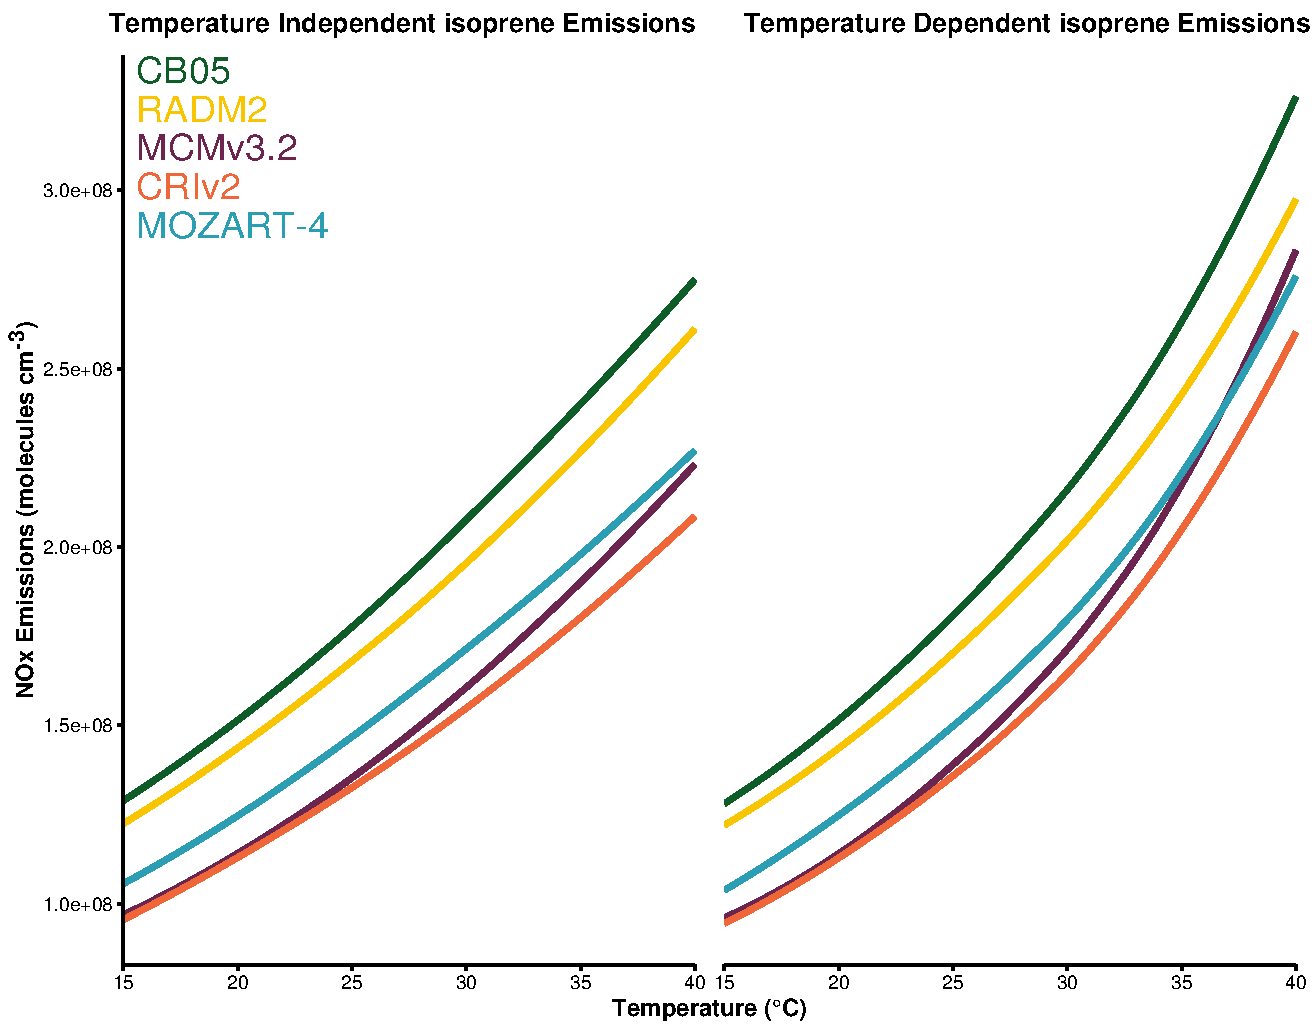
\includegraphics[width = 0.9\textwidth]{img/NOx_emissions_for_Maximal-O3}
\end{figure}

\begin{figure}[ht]
    \centering
    \caption{Contributions to cumulative VOC reactivity (VOCR) from different functional groups of emitted VOCs to the total VOCR. Results illustrated at each temperature, for each chemical mechanism and source of isoprene emissions (temperature-independent and temperature-dependent).}
    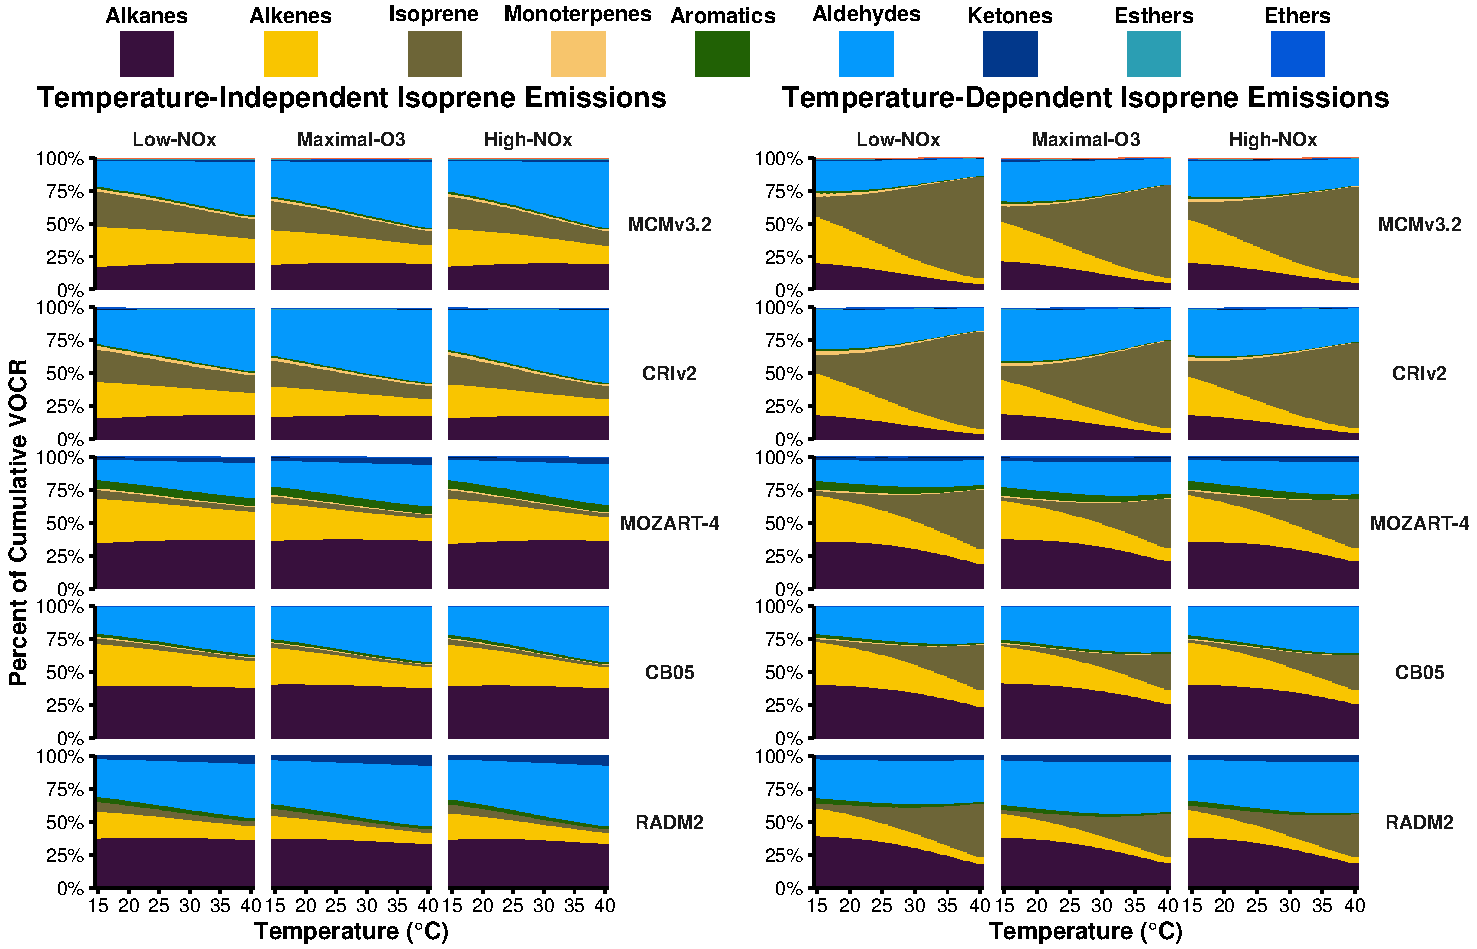
\includegraphics[width = 0.9\textwidth]{img/Sum_VOCR_percent}
\end{figure}

\newpage

\section{Ox Production and Consumption Budgets}
\vspace{-2mm}
Further box model simulations of stagnant conditions were performed as outlined in Section~3.3 of the research article and an analysis similar to that Section~3.2 of the research article looked at the production and consumption budgets of \ce{O_x} was performed.
As in Fig.~4 of the research article the production and consumption of \ce{O_x} are allocated to the net contributions of major categories: `ARO2', `RO2' and `HO2' represent the reaction of acyl peroxy radicals, alkyl peroxy radicals and \ce{HO2} with NO.
`Inorganic' represents the net contribution of inorganic reactions, `RO2NO2' the net contribution of peroxy nitrates and any other reactions were allocated to the `Other Organic' category.
The absolute \ce{O_x} production and consumption budgets for these addition simulations are depicted in Fig.~\ref{f:abs_Ox} while the \ce{O_x} budgets normalised by the total chemical loss rate of emitted VOC are displayed in Fig.~\ref{f:norm_Ox}.
These \ce{O_x} budgets are displayed for each chemical mechanism, \ce{NO_x} condition and source of isoprene emissions (temperature independent and temperature dependent) in Figs.~\ref{f:abs_Ox} and \ref{f:norm_Ox}.
This analysis support the conclusion that the increased OH-reactivity of the emitted VOCs caused the increase of ozone with temperature in our study.
\begin{figure}[ht]
    \centering
    \caption{Day-time budgets of \ce{O_x} from box model simulations without mixing allocated to the \ce{NO_x}-regimes allocated to the net contribution of reactions to \ce{O_x} budgets are allocated to categories of inorganic reactions, peroxy nitrates (RO2NO2), reactions of NO with HO2, alkyl peroxy radicals (RO2) and acyl peroxy radicals (ARO2). All other reactions are allocated to the 'Other Organic' category.}
    \begin{subfigure}[t]{\textwidth}
        \centering
        \caption{Absolute \ce{O_x} production and consumption budgets.}
        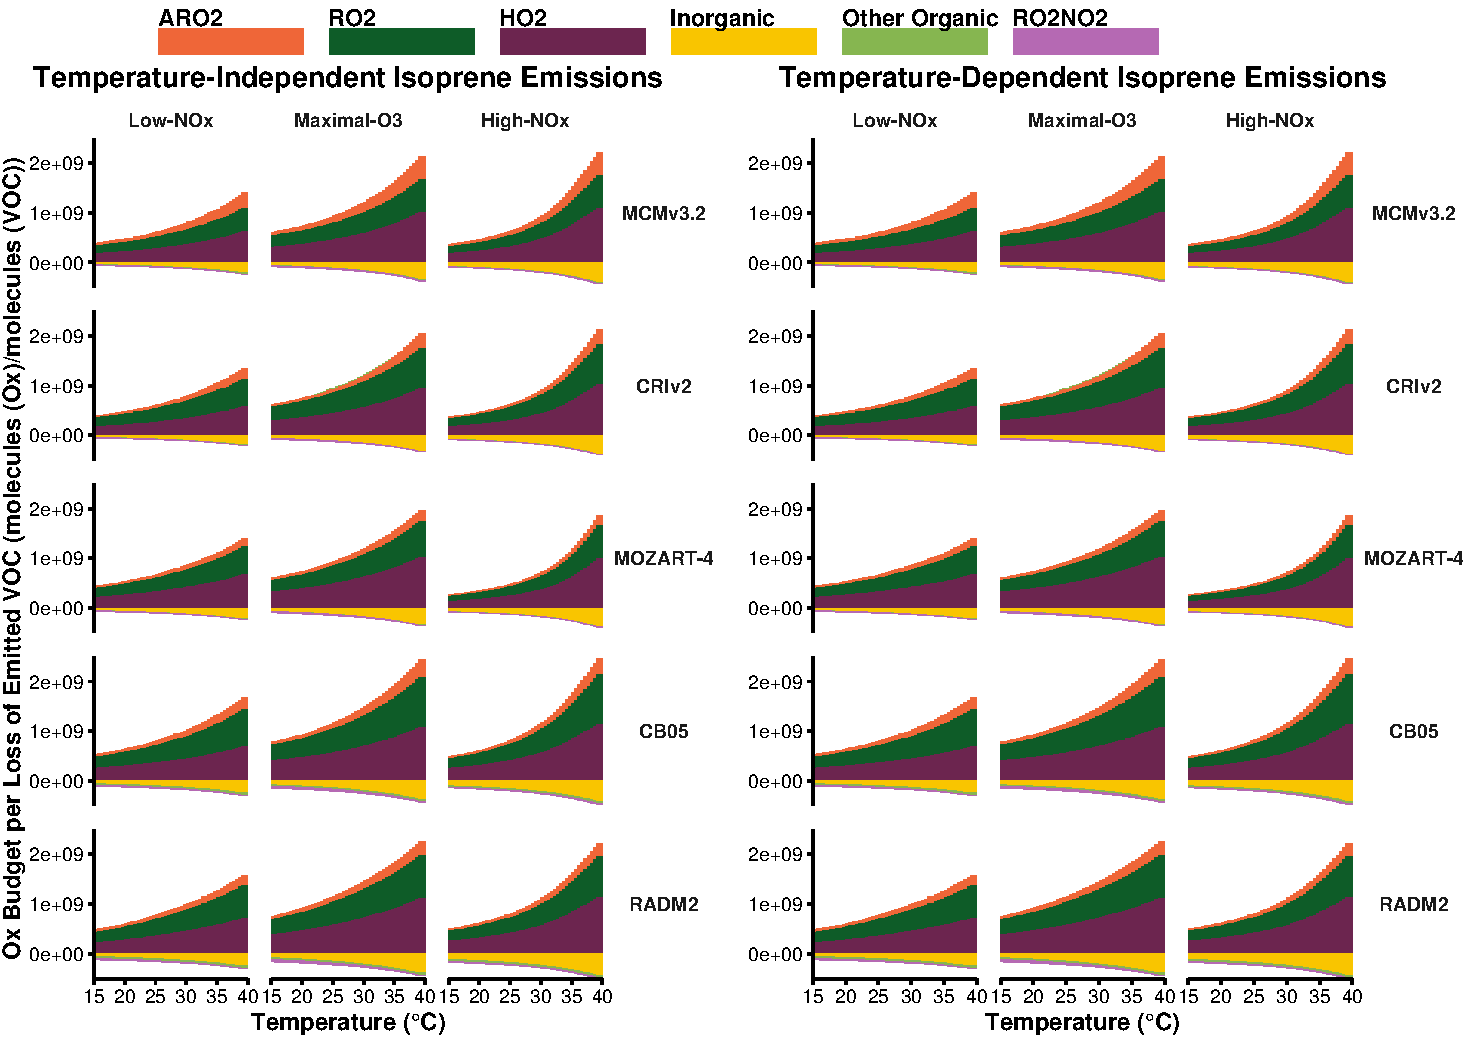
\includegraphics[width = 0.97\textwidth]{img/Absolute_Ox_Budget_categories-No_mixing}
        \label{f:abs_Ox}
    \end{subfigure}
    \\
    \begin{subfigure}[t]{\textwidth}
        \centering
        \caption{\ce{O_x} production and consumption budgets normalised by the total chemical loss rate of emitted VOC.}
        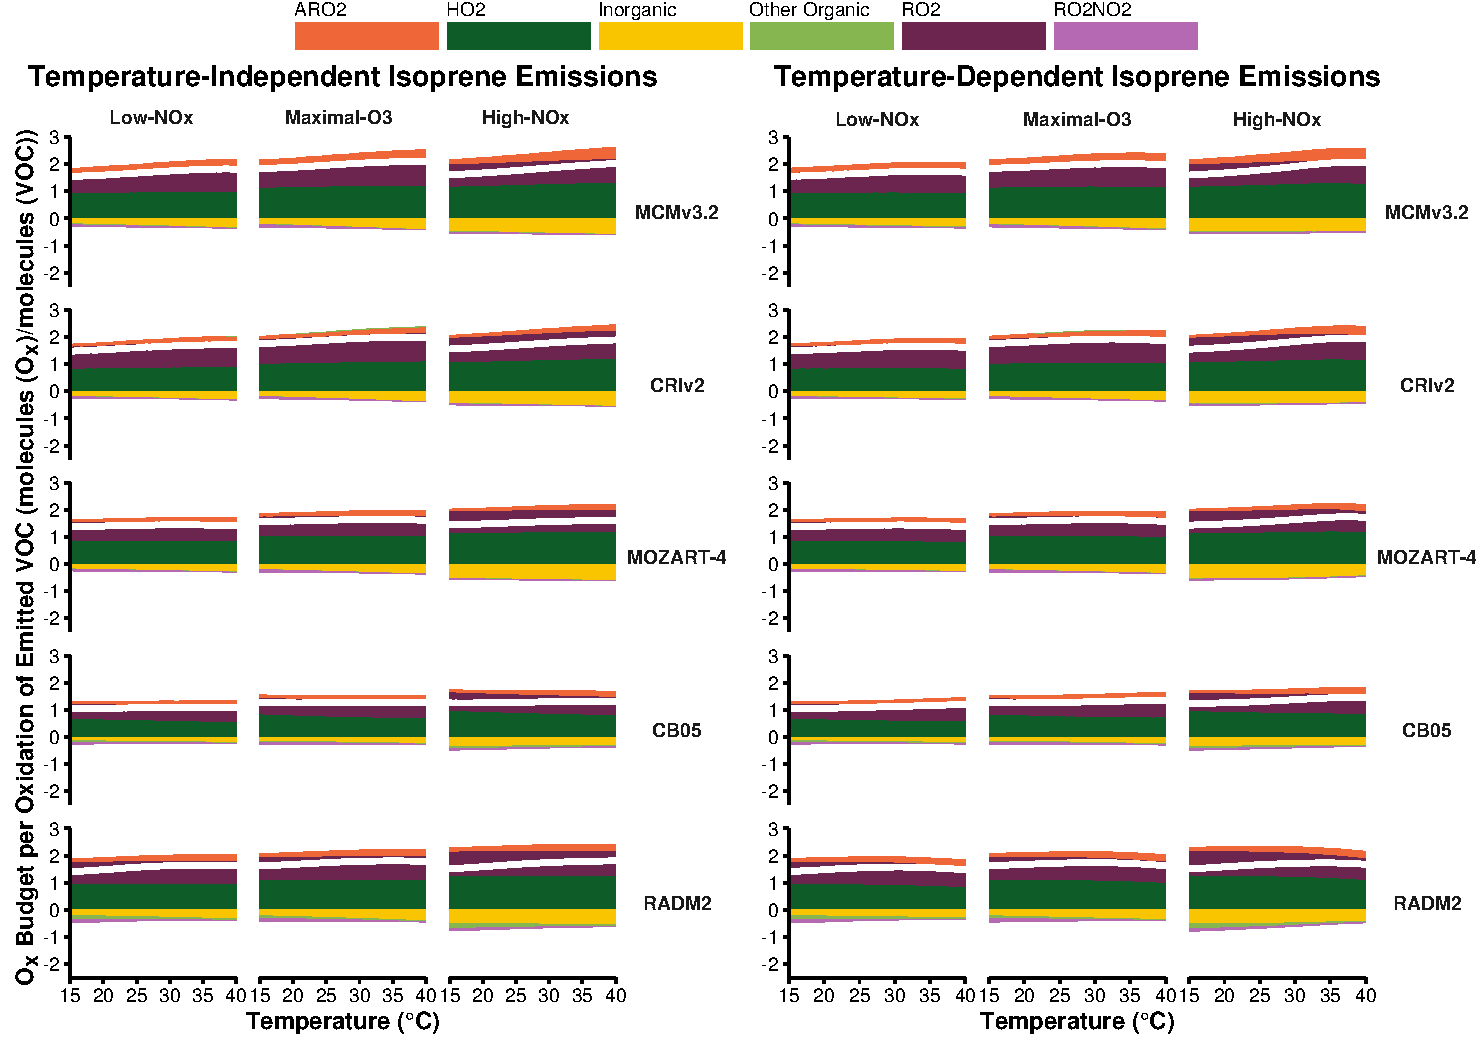
\includegraphics[width = 0.97\textwidth]{img/Normalised_Ox_Budget-No_mixing}
        \label{f:norm_Ox}
    \end{subfigure}
\end{figure}

\clearpage
\bibliographystyle{abbrvnat}
\bibliography{References} 

\end{document}
